\documentclass[11pt,reqno]{amsart}

\usepackage[margin=1.05in]{geometry}
\usepackage{amsmath,amssymb,amsthm,mathtools}
\usepackage{booktabs,array}
\usepackage{graphicx}
\usepackage{xcolor}
\usepackage{hyperref}

\definecolor{navy}{HTML}{0F172A}
\definecolor{accent}{HTML}{1D4ED8}
\hypersetup{
  colorlinks=true,
  linkcolor=accent,
  citecolor=accent,
  urlcolor=accent,
  pdftitle={Invisible Boundary Loads on Convex Polygons: Leont'ev's Exponential Lattice, Balayage Anatomy, and Fokas's Global Relation}
}

\newtheorem{theorem}{Theorem}[section]
\newtheorem{proposition}[theorem]{Proposition}
\newtheorem{lemma}[theorem]{Lemma}
\newtheorem{corollary}[theorem]{Corollary}
\theoremstyle{definition}
\newtheorem{definition}[theorem]{Definition}
\theoremstyle{remark}
\newtheorem{remark}[theorem]{Remark}

\newcommand{\C}{\mathbb{C}}
\newcommand{\R}{\mathbb{R}}
\newcommand{\Z}{\mathbb{Z}}
\newcommand{\N}{\mathbb{N}}
\DeclareMathOperator{\Log}{Log}
\DeclareMathOperator{\dist}{dist}
\DeclareMathOperator{\sgn}{sgn}
\DeclareMathOperator{\sinhc}{sinhc}

\title[Invisible Boundary Loads on Convex Polygons]{Invisible Boundary Loads on Convex Polygons:\\
Leont'ev's Exponential Lattice, Balayage Anatomy,\\
and Fokas's Global Relation}

\author{Project ReMath}
\date{November 23, 2026}
\subjclass[2020]{Primary 30B50, 30D15; Secondary 31A15, 35J05, 42C15}
\keywords{Exponential series, representing systems, convex polygons, A.~F.~Leont'ev, Fokas unified transform, harmonic balayage, Saint-Venant torsion, entire functions of exponential type}

\begin{document}

\begin{abstract}
Between 1965 and 1987, A.~F.~Leont'ev and his school developed a comprehensive theory of representing holomorphic functions on bounded convex domains $D \subset \C$ by non-orthogonal series of exponentials $\sum c_\nu e^{\nu z}$. On a convex $p$-gon $D$, the canonical exponents form a semi-infinite lattice $\Lambda_+$ supported on the $p$ spectral rays $\mathcal{R}_j = \R_+(i/d_j)$ conjugate to the outward normals of $D$---the exact spectral rays later employed in A.~S.~Fokas's Unified Transform Method for boundary value problems on polygons. In this paper we establish a direct analytical bridge between these two traditions and solve the dual annihilation problem: characterizing all real boundary loads $\mu$ on $\partial D$ whose exponential transform $B_\mu(s) = \int_{\partial D} e^{sw}\,d\mu(w)$ vanishes on $\Lambda_+$.

First, we prove an explicit contour-residue formula converting Fokas's continuous ray transforms into the canonical discrete Leont'ev coefficients, analyze an explicit meromorphic ``ghost wave'' on the square whose Lambert continuation cancels outside the domain despite exponential ray divergence, and establish the sharp erasure criterion $\#\{\nu \in E : |\nu|\le R\} = o(R)$ alongside zero $\ell^2$ coefficient infima and $\ell^1$ non-attainment for $F \equiv 1$. Second, for \emph{every} genuine convex $p$-gon ($p \ge 3$), we determine the exact real dimensions of the one-sided invisible kernels in $(L^2(\partial D), L^1(\partial D), \mathcal{M}(\partial D))$: they equal $(2k-1, 2k+1, 2k+1)$ when $p = 2k+1$---exhibiting a two-dimensional $L^1 \setminus L^2$ corner-singularity gap---and $(2k-1, 2k-1, 2k)$ when $p = 2k$, invariant under arbitrary non-parallel vertex perturbations. On the two-sided lattice $\Lambda_\pm$, all nonzero real invisible measures collapse to dimension zero the instant central symmetry is broken. Third, we prove that Saint-Venant's uniform torsion shear stress $-\partial_n u$ ($-\Delta u = 1$, $u|_{\partial D}=0$) belongs to the invisible $L^2$ kernel if and only if $D$ is a parallelogram ($p=4$), whereas on a general centrally symmetric $2k$-gon ($k \ge 2$) the canonical invisible flux is the harmonic balayage $-\partial_n u_{\mathrm{box}}$ of the zonotope probability box-spline density ($-\Delta u_{\mathrm{box}} = M_{d_1,\dots,d_k}$). On the unit equilateral triangle, uniform torsion fails at the first node, and the unique mass-one invisible $L^2$ boundary flux $g_\triangle$ is the Poisson balayage of a strictly positive one-dimensional probability measure on the three-spoked median skeleton, governed by Binet's log-Gamma kernel ($\zeta(6m+4)$) with corner law $g_\triangle(x) = \sqrt{2/\pi}\,x^{1/2} + O(x^2)$. Finally, we identify the $L^2$ invisible kernel with the nullspace of full integer-lattice Global Relation collocation for Laplace's equation and prove that appending $2k-1$ boundary moments removes the nullspace, illustrated to machine precision in an enriched solver. Core algebraic symmetry and Vandermonde grouping lemmas are formally verified in Lean~4.
\end{abstract}

\maketitle

\section{Introduction}

Let $D \subset \C$ be a bounded convex domain. Whereas power series $\sum a_n z^n$ converge naturally on disks and classical Fourier series $\sum c_n e^{inx}$ operate on intervals, A.~F.~Leont'ev discovered in a landmark sequence of works \cite{Leontev1969UMN,Leontev1969MatSb,Leontev1973Izv,Leontev1974Polygon,Leontev1976Book,Leontev1987TrMIAN} that \emph{every} function holomorphic in $D$ expands in an absolutely convergent series of exponentials $\sum_{n=1}^\infty c_n e^{\lambda_n z}$ whose exponents $\{\lambda_n\}$ depend only on the geometry of $D$. Unlike an orthogonal Schauder basis, such an exponential system is inherently overcomplete: under the canonical-symbol condition $Q_1$ (an entire function of indicator bounded by the domain support function having $\{\lambda_n\}$ as simple zeros), Yu.~F.~Korobeinik \cite[Ch.~III, \S 1, Theorem~6]{Korobeinik1981UMN} (cf.\ \cite{Korobeinik1975}) proved that $\{e^{\lambda_n z}\}$ forms an absolutely representing system in $H(D)$ if and only if $H(D)$ admits a \emph{nontrivial expansion of zero} $\sum_{n=1}^\infty c_n e^{\lambda_n z} \equiv 0$. Because Leont'ev's foundational 536-page monograph \emph{Series of Exponentials} (\emph{Ryady eksponent}, 1976) \cite{Leontev1976Book} and its sequels were never translated into English, much of this geometric apparatus remained isolated from Western developments in boundary value problems and computational harmonic analysis.

Three decades after Leont'ev's polygon theorems, A.~S.~Fokas introduced the Unified Transform Method for linear and integrable partial differential equations \cite{FokasBook2008}, developed rigorously on convex polygons by Fulton, Fokas, and Xenophontos \cite{FFX2004} and Ashton and Fokas \cite{Ashton2012,AshtonFokas2013}. For Laplace's equation $\Delta q = 0$ on a convex $p$-gon $D$ with counterclockwise vertices $\gamma_1, \dots, \gamma_p$ and edge vectors $d_j = \gamma_{j+1}-\gamma_j$ ($\gamma_{p+1}=\gamma_1$), any holomorphic derivative $F = \partial_z q \in H(D) \cap C(\bar D)$ admits the continuous integral representation
\begin{equation}\label{eq:fokas-rep}
  F(z) = \frac{1}{2\pi} \sum_{j=1}^p \int_{\ell_j} e^{i\lambda z} \rho_j(\lambda)\,d\lambda,
  \qquad \rho_j(\lambda) = \int_{\Gamma_j} e^{-i\lambda w} F(w)\,dw,
\end{equation}
along the outward rays $\ell_j = \{r e^{-i\arg d_j} : r \ge 0\}$, coupled by the \emph{Global Relation} $\sum_{j=1}^p \rho_j(\lambda) = 0$ ($\lambda \in \C$). Under the spectral rotation $s = i\lambda$, the Fokas integration rays $\mathcal{R}_j = \R_+(i/d_j)$ coincide \emph{identically} with the spectral rays carrying Leont'ev's canonical polygon lattice
\begin{equation}\label{eq:lattice-def}
  \Lambda_+ = \left\{ \nu_{jm} = m b_j : 1 \le j \le p,\; m \in \Z_{\ge 1} \right\},
  \qquad b_j = \frac{2\pi i}{d_j}, \quad c_j = \frac{1}{b_j} = \frac{d_j}{2\pi i}.
\end{equation}
(Note that in the exponential pairing $\operatorname{Re}(sw)$, the physical outward unit normal to $\Gamma_j$ is $\bar b_j/|b_j| = -i d_j/|d_j|$, while $b_j$ is its complex conjugate.)

This coincidence raises two fundamental questions that motivate the present paper:
\begin{enumerate}
  \item \emph{Synthesis bridge}: How does Fokas's continuous outward-ray transform \eqref{eq:fokas-rep} pass analytically into Leont'ev's discrete decomposition $F(z) = \sum_{j=1}^p F_j(z)$ into $p$ edge-periodic half-plane waves, and what is the structure of the synthesis nullspace and frequency-erasure threshold?
  \item \emph{Dual annihilation (invisible loads)}: Given the boundary exponential transform
  \begin{equation}\label{eq:B-def}
    B_\mu(s) = \int_{\partial D} e^{sw}\,d\mu(w)
  \end{equation}
  of a real boundary measure or flux density on $\partial D$, which nonzero real loads satisfy $B_\mu(\nu) = 0$ for \emph{every} $\nu \in \Lambda_+$ (or on the two-sided lattice $\Lambda_\pm = \Lambda_+ \cup (-\Lambda_+)$)? What are these ``invisible physical loads'' explicitly, and how do they govern the nullspace of Leont'ev-lattice Global Relation collocation?
\end{enumerate}

\subsection*{Summary of main results}
Throughout, $D \subset \C$ denotes a bounded positive-area convex $p$-gon ($p \ge 3$) presented by its genuine counterclockwise vertices $\gamma_1,\dots,\gamma_p$, meaning every interior angle satisfies $0 < \omega_j < \pi$. (Artificially subdividing a straight edge alters $\Lambda_+$.)

\begin{table}[ht]
\centering
\caption{Exact real dimensions of the invisible boundary-load kernels $\mathcal{K}_X(\Lambda_+)$ and $\mathcal{K}_{\mathcal{M}}(\Lambda_\pm)$ on an arbitrary genuine convex $p$-gon $D \subset \C$.}
\label{tab:dimensions}
\footnotesize
\begin{tabular}{lrrrr}
\toprule
Polygon class & $\dim_\R \mathcal{K}_{L^2}$ & $\dim_\R \mathcal{K}_{L^1}$ & $\dim_\R \mathcal{K}_{\mathcal{M}}(\Lambda_+)$ & $\dim_\R \mathcal{K}_{\mathcal{M}}(\Lambda_\pm)$ \\
\midrule
Triangle ($p=3$, equilateral or scalene) & $1$ & $3$ & $3$ & $0$ \\
Non-parallel quadrilateral ($p=4$) & $3$ & $3$ & $4$ & $0$ \\
Trapezoid (one parallel pair, $p=4$) & $3$ & $3$ & $4$ & $0$ \\
Parallelogram / square ($p=4$) & $3$ & $3$ & $4$ & $4$ \\
Pentagon ($p=5$) & $3$ & $5$ & $5$ & $0$ \\
General odd $p = 2k+1$ ($k \ge 1$) & $2k-1$ & $2k+1$ & $2k+1$ & $0$ \\
General even $p = 2k$ ($k \ge 2$) & $2k-1$ & $2k-1$ & $2k$ & $2k$ (cent.\ sym.) / $0$ \\
\bottomrule
\end{tabular}
\end{table}

\begin{itemize}
  \item \textbf{Continuous-to-discrete transfer, meromorphic ghosts, and erasure (Section~\ref{sec:bridge})}: Theorem~\ref{thm:bridge} gives an exact contour-residue integral for the canonical Leont'ev coefficients $c_\nu$ via all $p$ Fokas ray transforms $R_j(s)$, explaining why single-edge sampling fails even for $F \equiv 1$. Theorem~\ref{thm:ghost-erasure} exhibits a closed-form ghost wave on the square whose Lambert continuation cancels across all four rotations outside $D$, proves the sharp erasure threshold $\#\{\nu \in E : |\nu|\le R\} = o(R)$, and shows via Hahn--Banach and P\'olya--Valiron that $\inf \|c\|_2 = 0$ (unattained for $F \not\equiv 0$) and $\inf \|c\|_1 = |F(0)|$ (unattained whenever $F(0)\ne 0$ and $F^{(4)}(0)=0$, e.g.\ $F \equiv 1$).
  \item \textbf{Universal classification of invisible boundary loads (Section~\ref{sec:classification})}: Theorem~\ref{thm:invisible-table} proves Table~\ref{tab:dimensions} for every convex $p$-gon. On odd polygons ($p=2k+1$), no nonzero pure-atom invisible load exists, yet two integrable modes lie in $L^q(\partial D)$ ($1 \le q < 2$) and fail local $L^2$ integrability at the vertices (mirroring Sedletskii's endpoint phenomenon for periodic projections \cite{Sedletskii1978,Sedletskii1988}). On even polygons ($p=2k$), an extra measure mode carrying alternating corner charges persists even when no two edges are parallel, compensated by an $L^2(\partial D, \R)$ density. On $\Lambda_\pm$, Theorem~\ref{thm:two-sided} proves that breaking central symmetry collapses $\mathcal{K}_{\mathcal{M}}(\Lambda_\pm)$ to $\{0\}$.
  \item \textbf{Saint-Venant torsion, zonotope box splines, and the triangle's median skeleton (Section~\ref{sec:anatomy})}: Theorem~\ref{thm:torsion} proves that uniform Saint-Venant torsion shear stress $-\partial_n u$ ($-\Delta u = 1$, $u|_{\partial D}=0$) lies in $\mathcal{K}_{L^2}(\Lambda_+)$ \emph{if and only if} $D$ is a parallelogram ($p=4$), while on every centrally symmetric $2k$-gon ($k \ge 2$) the canonical symbol $L(s)$ is the moment generating function of the polygon's zonotope probability box spline \cite{BoxSplines}, whose harmonic balayage generalizes torsion to $k \ge 3$. On the unit equilateral triangle, uniform torsion fails at $m=1$, and Theorem~\ref{thm:triangle-skeleton} proves via Binet's exact remainder and Phragm\'en--Lindel\"of that the unique mass-one invisible $L^2$ boundary density $g_\triangle$ is the Poisson balayage of a strictly positive 1D probability measure supported on the three vertex-to-centroid segments, with radial series governed by $\zeta(6m+4)$ and corner asymptotic $g_\triangle(x) = \sqrt{2/\pi}\,x^{1/2} + O(x^2)$.
  \item \textbf{Fokas Global Relation completion and Lean~4 verification (Section~\ref{sec:fokas})}: Theorem~\ref{thm:fokas-completion} identifies $\mathcal{K}_{L^2}(\Lambda_+)$ with the exact nullspace of full integer-lattice Global Relation collocation at fixed Dirichlet trace and proves that appending the mass and complex moments of degrees $1,\dots,k-1$ yields an injective lower-triangular completion. Companion bandlimited minimax and super-resolution laws for corner-atom recovery are treated in a separate paper \cite{Paper2}.
\end{itemize}

\section{The Gamma-Product Symbol and Uniform Asymptotics}\label{sec:symbol}

Let $D \subset \C$ have counterclockwise vertices $\gamma_1,\dots,\gamma_p$ ($p \ge 3$), edge vectors $d_j = \gamma_{j+1}-\gamma_j$, and Euclidean support function in the exponential-transform convention
\[
  H(s) = \max_{w \in \bar D} \operatorname{Re}(s w), \qquad s \in \C.
\]
Thus every finite complex Borel measure $\mu$ on $\bar D$ satisfies $|B_\mu(s)| \le \|\mu\|_{\mathrm{TV}} e^{H(s)}$. Observe that $\sum_{j=1}^p c_j = (2\pi i)^{-1}\sum_{j=1}^p d_j = 0$, and since all interior angles are strictly less than $\pi$, the spectral rays $\mathcal{R}_j = \R_+ b_j$ ($1 \le j \le p$) are pairwise distinct even when $D$ possesses parallel opposite sides ($d_{j+k} = -d_j$ gives $b_{j+k} = -b_j$).

\begin{definition}[Canonical Gamma-product symbol]\label{def:L}
Fix a unit complex number $u \notin \bigcup_{j=1}^p \R_+ b_j$ that strictly exposes a unique vertex $v$ of $D$, i.e., $\operatorname{Re}(u v) > \operatorname{Re}(u w)$ for all $w \in \bar D \setminus \{v\}$. With $\Log$ denoting the principal branch on $\C \setminus (-\infty,0]$, define
\begin{equation}\label{eq:L-def}
  \tau = v - \sum_{j=1}^p c_j \Log(-c_j u), \qquad
  L(s) = e^{\tau s} \prod_{j=1}^p \Gamma(1 - c_j s)^{-1}.
\end{equation}
\end{definition}

Whereas Leont'ev \cite{Leontev1974Polygon,Leontev1987TrMIAN} constructs odd-polygon canonical products via a half-shifted auxiliary grid followed by single-node deletion, the inverse-Gamma product \eqref{eq:L-def} is our chosen full-grid normalization: it retains \emph{every} positive integer node on every spectral ray, satisfies $L(0) = 1$, and has simple zeros precisely at $\Lambda_+$.

\begin{lemma}[Well-definedness and global two-sided bounds]\label{lem:L-bounds}
The drift vector $\tau$ and entire function $L(s)$ in \eqref{eq:L-def} are independent of the choice of exposing direction $u$. Setting $h = p/2$, we have:
\begin{enumerate}
  \item \emph{Open sectors}: Uniformly as $R \to \infty$ for $u$ in any compact subset of $S^1 \setminus \{b_j/|b_j|\}_{j=1}^p$ exposing vertex $v$,
  \begin{equation}\label{eq:sector-asymp}
    L(R u) = A(u) R^{-h} e^{R u v}\bigl(1 + O(R^{-1})\bigr),
    \qquad A(u) = (2\pi)^{-h} \exp\!\left(-\frac{1}{2}\sum_{j=1}^p \Log(-c_j u)\right).
  \end{equation}
  \item \emph{Ray transition cones}: In a sufficiently small closed angular sector about ray $\mathcal{R}_j$, choosing a continuous branch of $s^{-h}$ across the ray gives a nonzero constant $C_{\gamma_j}$ such that uniformly as $|s|\to\infty$,
  \begin{equation}\label{eq:ray-asymp}
    L(s) = C_{\gamma_j} s^{-h} e^{s\gamma_j}(1 - e^{s d_j})\bigl(1 + O(|s|^{-1})\bigr).
  \end{equation}
  Moreover, along the boundary of $D$, the vertex constants on a continuous angular branch alternate in sign across each ray: if $p = 2k$ is even, $s^{-h} = s^{-k}$ is single-valued and $C_{\gamma_{j+1}} = -C_{\gamma_j}$ for all $j$.
  \item \emph{Uniform global estimate}: Uniformly for all $|s| \ge 1$,
  \begin{equation}\label{eq:global-L}
    |L(s)| \asymp_D e^{H(s)} (1 + |s|)^{-h} \min\bigl\{1, \dist(s, \Lambda_+)\bigr\},
    \qquad |L'(\nu)| \asymp_D e^{H(\nu)} (1 + |\nu|)^{-h} \quad (\nu \in \Lambda_+).
  \end{equation}
\end{enumerate}
\end{lemma}

\begin{proof}
For $u \in S^1$ away from the rays $\R_+ b_j$, none of the points $-c_j R u$ lies on $(-\infty,0]$. Stirling's expansion $\log \Gamma(1+z) = (z+\frac12)\Log z - z + \frac12\log(2\pi) + O(|z|^{-1})$ applied to $z = -c_j R u$ and summed over $j = 1,\dots,p$ cancels both $(R\log R)\sum c_j = 0$ and the linear $-R u \sum c_j = 0$ terms, yielding
\[
  \sum_{j=1}^p \log \Gamma(1 - c_j R u)^{-1}
  = R u \sum_{j=1}^p c_j \Log(-c_j u) - h \log R - h\log(2\pi) - \frac{1}{2}\sum_{j=1}^p \Log(-c_j u) + O(R^{-1}).
\]
Adding $\tau R u$ gives \eqref{eq:sector-asymp}. Within each open sector between consecutive rays, $u \mapsto \sum_j c_j \Log(-c_j u)$ has angular derivative zero since $\sum_j c_j = 0$, hence is locally constant. For $u(\delta) = b_j e^{i\delta}/|b_j|$, $-c_j u(\delta) = -e^{i\delta}/|b_j|$ has imaginary part $-\sin\delta/|b_j|$, crossing $(-\infty,0)$ from the upper half-plane ($\delta < 0$) to the lower half-plane ($\delta > 0$). Thus $\Log(-c_j u(\delta))$ jumps by $-2\pi i$ as $\delta$ crosses $0$ from negative to positive, so $-\sum_\ell c_\ell \Log(-c_\ell u(\delta))$ jumps by $+2\pi i c_j = d_j$. Simultaneously, $b_j e^{i\delta}(-d_j) = 2\pi\sin\delta - 2\pi i\cos\delta$ has negative real part for $\delta < 0$ and positive real part for $\delta > 0$, meaning the exposed vertex switches from $\gamma_{j+1}$ ($\delta < 0$) to $\gamma_j = \gamma_{j+1} - d_j$ ($\delta > 0$). Hence $v(\delta) - \sum_\ell c_\ell \Log(-c_\ell u(\delta))$ is invariant across every ray, proving that $\tau$ is independent of $u$ and $\operatorname{Re}(R u v) = H(R u)$ on every open sector.

Near ray $\mathcal{R}_j$, Euler's reflection identity $\Gamma(1 - c_j s)^{-1} = \pi^{-1}\Gamma(c_j s)\sin(\pi c_j s)$ and $2\pi i c_j = d_j$ give $\sin(\pi c_j s) = -\frac{1}{2i} e^{-s d_j/2}(1 - e^{s d_j})$. Applying Stirling's formula to $\Gamma(c_j s)$ and to $\Gamma(1 - c_\ell s)^{-1}$ ($\ell \ne j$) in a small cone around $\mathcal{R}_j$ gives \eqref{eq:ray-asymp}. For $\delta > 0$ ($\operatorname{Re}(s d_j) < 0$), $1 - e^{s d_j} \to 1$ gives leading term $C_{\gamma_j} s^{-h} e^{s\gamma_j}$, while for $\delta < 0$ ($\operatorname{Re}(s d_j) > 0$), $e^{s\gamma_j}(1 - e^{s d_j}) \sim -e^{s\gamma_{j+1}}$, confirming $C_{\gamma_{j+1}} = -C_{\gamma_j}$ along a continuous branch of $s^{-h}$. Finally, on the strip $|\operatorname{Re}(s d_j)| \le 1$, $|e^{s\gamma_j}(1 - e^{s d_j})| \asymp e^{H(s)}\min\{1,\dist(s,\Lambda_+)\}$, while outside that strip one of $1$ or $e^{s d_j}$ dominates uniformly, giving the first bound in \eqref{eq:global-L}. Setting $r_0 = \frac14\inf_{\nu\ne\nu'\in\Lambda_+} |\nu - \nu'| > 0$, dividing the two-sided bound for $|L(s)|$ by $|s - \nu|$ on $0 < |s - \nu| \le r_0$, and letting $s \to \nu$ yields the derivative estimate in \eqref{eq:global-L}.
\end{proof}

\section{Exact Fokas--Leont'ev Transfer, Ghost Waves, and Erasure}\label{sec:bridge}

On a convex $p$-gon $D$, Fokas's representation \eqref{eq:fokas-rep} becomes, in the variable $s = i\lambda$ ($ds = i\,d\lambda$),
\begin{equation}\label{eq:fokas-s}
  F(z) = \frac{1}{2\pi i} \sum_{j=1}^p \int_{\mathcal{R}_j} e^{sz} R_j(s)\,ds,
  \qquad R_j(s) = \int_{\Gamma_j} e^{-sw} F(w)\,dw, \quad z \in D.
\end{equation}

One might naively guess that the residue-selected coefficient $c_{\nu_{jm}}$ along ray $j$ is obtained directly from the single-edge sample $R_j(\nu_{jm})$. The constant function $F \equiv 1$ immediately refutes this: for every $m \ge 1$, $R_j(\nu_{jm}) = \int_{\Gamma_j} e^{-m b_j w}\,dw = -d_j(2\pi i m)^{-1} e^{-m b_j \gamma_j}(e^{-2\pi i m} - 1) = 0$. Every own-edge sample vanishes identically! Instead, the canonical discrete coefficients couple \emph{all} $p$ continuous rays.

\begin{theorem}[Continuous-to-discrete residue transfer]\label{thm:bridge}
Let $F \in H(D) \cap C(\bar D)$, and let $L(s)$ be the canonical Gamma-product symbol \eqref{eq:L-def}. Then for every $z \in D$,
\begin{equation}\label{eq:transfer}
  F(z) = \sum_{\nu \in \Lambda_+} c_\nu e^{\nu z}, \qquad
  c_\nu = \frac{1}{2\pi i L'(\nu)} \sum_{j=1}^p \int_{\mathcal{R}_j} \frac{L(s) R_j(s)}{s - \nu}\,ds,
\end{equation}
where the series converges absolutely and locally uniformly in $D$, and each ray integral is absolutely convergent (with a removable singularity at $s = \nu$ when $\nu \in \mathcal{R}_j$). When $F$ extends holomorphically to a neighborhood of $\bar D$, $\frac{1}{2\pi i}\sum_{j=1}^p \int_{\mathcal{R}_j} \frac{L(s)R_j(s)}{s-\nu}\,ds$ coincides with Leont'ev's classical interpolating functional $\omega_L(\nu, F)$.
\end{theorem}

\begin{proof}
Fix a compact set $K \subset D$; then $\max_{z \in K}\operatorname{Re}(sz) \le H(s) - \delta |s|$ for some $\delta > 0$. Because $\Lambda_+$ has bounded radial density, there exist circles $|s| = R_n \uparrow \infty$ staying at uniform positive distance from $\Lambda_+$. For fixed $s \notin \Lambda_+$ and $z \in K$, applying Cauchy's residue theorem to $\zeta \mapsto \frac{e^{\zeta z}}{(s-\zeta)L(\zeta)}$ on $|\zeta| = R_n$ yields, via \eqref{eq:global-L}, an outer boundary integral bounded by $C R_n^{h} e^{-\delta R_n} \to 0$. Hence
\begin{equation}\label{eq:kernel-res}
  e^{sz} = \sum_{\nu \in \Lambda_+} \frac{L(s) e^{\nu z}}{(s - \nu) L'(\nu)},
\end{equation}
which extends across $s \in \Lambda_+$ by continuity since $L(\nu) = 0$. Along ray $\mathcal{R}_j$, $H(s) = \operatorname{Re}(s\gamma_j) = \operatorname{Re}(s\gamma_{j+1})$, so $|R_j(s)| \le |d_j|\,\|F\|_\infty e^{-H(s)}$ with $\|F\|_\infty = \|F\|_{C(\bar D)}$. Combining this with \eqref{eq:global-L} gives $|L(s) R_j(s)| \le C_D \|F\|_\infty (1 + |s|)^{-p/2}$. Since $p \ge 3$, $p/2 \ge 3/2$, so for each $\nu \in \Lambda_+$ the quotient $(1+|s|)^{-p/2}/(1+|s-\nu|)$ lies in $L^1(\mathcal{R}_j)$ (using the simple zero of $L$ at $s = \nu$ for $|s-\nu| < r_0$). Moreover, summing over $\nu \in \Lambda_+$ for $z \in K$ yields
\[
  \sum_{\nu \in \Lambda_+} \frac{|e^{\nu z}|}{|L'(\nu)|(1+|s-\nu|)} \le C_K
\]
uniformly in $s \in \bigcup_j \mathcal{R}_j$ since $|e^{\nu z}/L'(\nu)| \le C |\nu|^h e^{-\delta|\nu|}$. Fubini's theorem in \eqref{eq:fokas-s}--\eqref{eq:kernel-res} establishes \eqref{eq:transfer}. Finally, for $F(w) = e^{a w}$ ($a \in \C \setminus \Lambda_+$), $\sum_{j=1}^p R_j(s)$ vanishes by Cauchy's theorem, while rotating the ray contours around $a$ evaluates the unnormalized ray sum in \eqref{eq:transfer} to $L(a)/(a-\nu)$, matching $\omega_L(\nu, e^{a\,\cdot})$ \cite{Leontev1969MatSb}; equality for all $F$ holomorphic near $\bar D$ follows by polynomial approximation.
\end{proof}

\begin{figure}[ht]
\centering
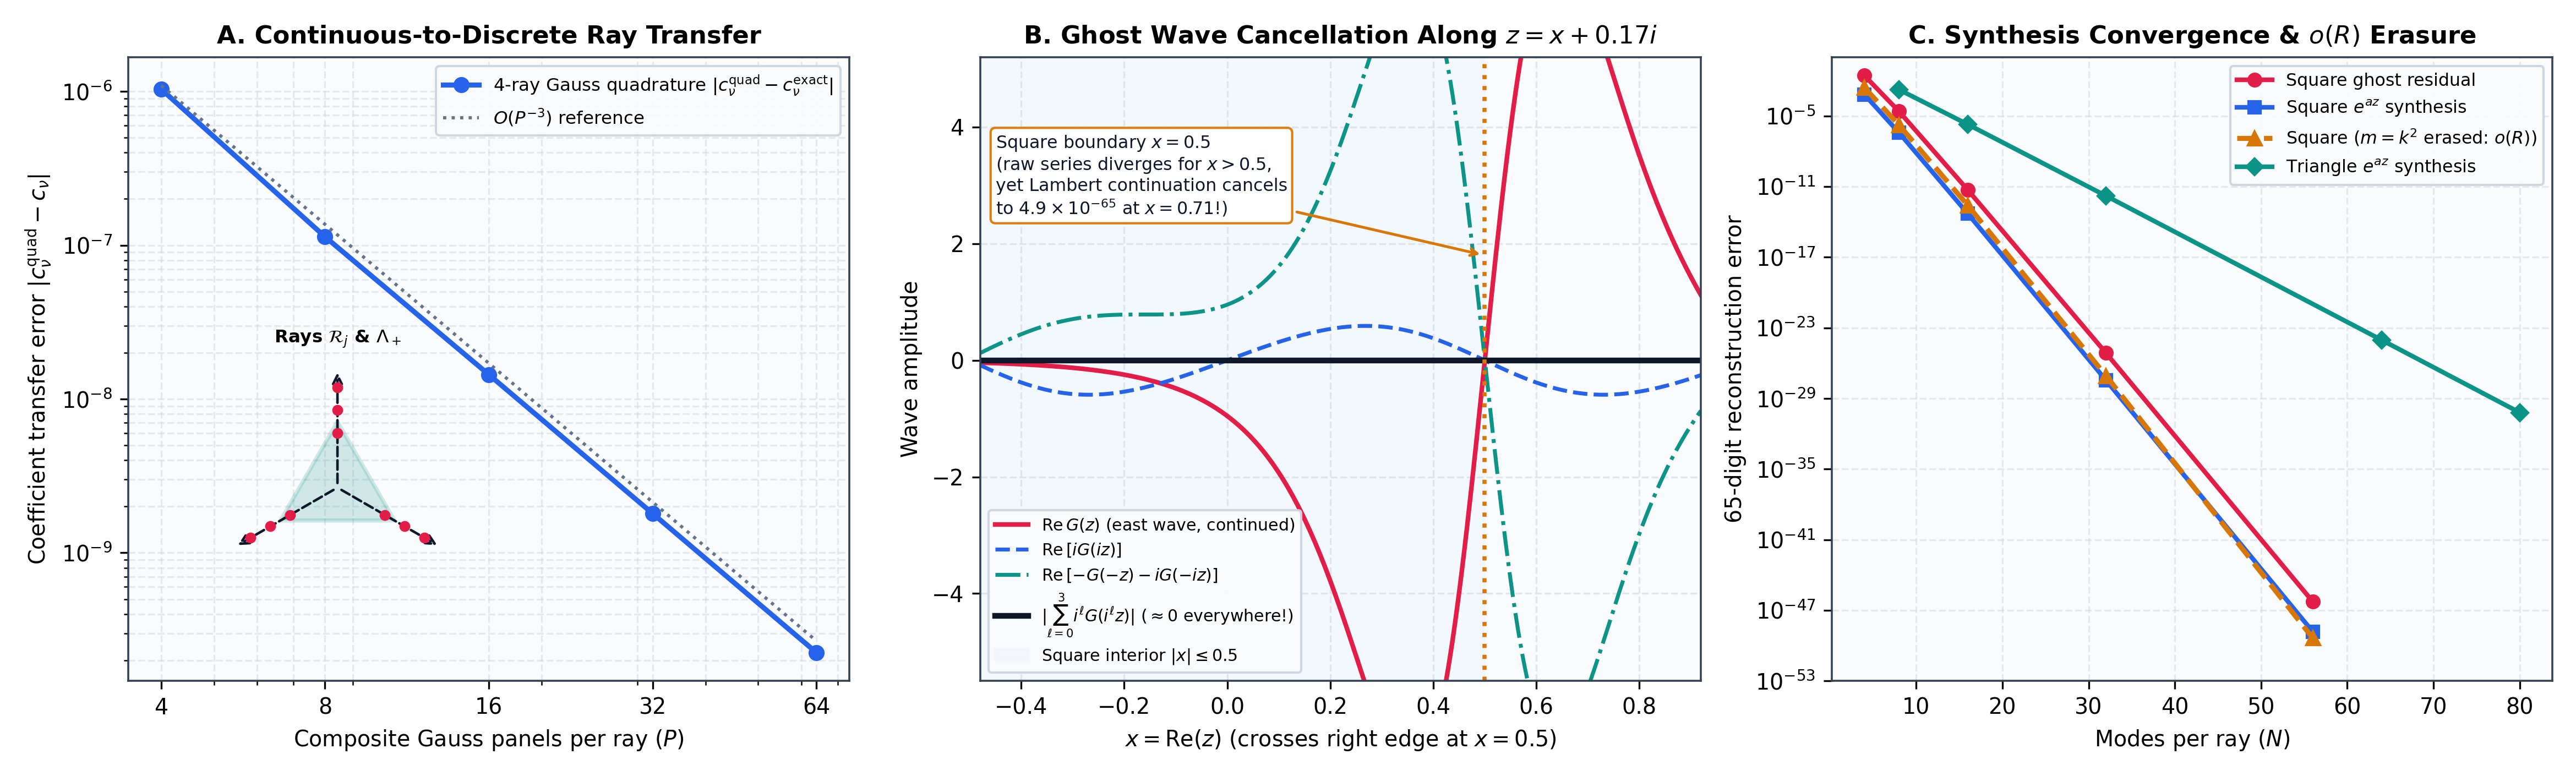
\includegraphics[width=\textwidth]{figs/p1_fig1_bridge_and_ghosts.png}
\caption{\textbf{A.} Convergence of composite 24-point Gauss quadrature on the four continuous Fokas rays to the residue-selected Leont'ev coefficient on the unit square ($2.24\times 10^{-10}$ at 64 panels). \textbf{B.} Analytic continuation of the four rotated ghost waves along the pole-free horizontal line $z = x + 0.17i$ across the right edge $x=0.5$: individual waves diverge in raw series outside $D$ (e.g.\ the single $m=40$ east term reaches $5.27\times 10^{27}$ at $x=0.71$), while the four-term Lambert continuation vanishes identically ($4.89\times 10^{-65}$ numerical residual). \textbf{C.} 65-digit truncation convergence on the square and equilateral triangle ($5.52\times 10^{-47}$ ghost residual at $z=0.17+0.13i$, $N=56$), including reconstruction of $F \equiv 1$ to $4.45\times 10^{-50}$ after erasing all square-indexed modes $m = k^2$ on an edge.}
\label{fig:bridge-ghosts}
\end{figure}

We next record the explicit structure of the synthesis kernel (``ghost waves''), its exterior meromorphic continuation, the sharp erasure law, and the failure of naive norm-minimization compression.

\begin{theorem}[Ghost waves, meromorphic continuation, sharp erasure, and norm collapse]\label{thm:ghost-erasure}
Let $D$ be a genuine convex $p$-gon with lattice $\Lambda_+$ and symbol $L(s)$.
\begin{enumerate}
  \item \emph{Ghost characterization and square Lambert continuation}: Sequence $(c_\nu)_{\nu \in \Lambda_+}$ satisfies $\sum_{\nu \in \Lambda_+} |c_\nu| |e^{\nu z}| < \infty$ locally uniformly in $D$ and $\sum_{\nu \in \Lambda_+} c_\nu e^{\nu z} \equiv 0$ on $D$ if and only if $c_\nu = A(\nu)/L'(\nu)$ for an entire function $A$ of minimal exponential type ($|A(s)| \le C_\varepsilon e^{\varepsilon|s|}$ for every $\varepsilon > 0$). On the centered unit square $[-\frac12,\frac12]^2$ with $L_{\mathrm{sq}}(s) = \sinhc(s/2)\sinhc(is/2)$, choosing $A \equiv 1$ gives $\sum_{\ell=0}^3 i^\ell G(i^\ell z) = 0$ on $D$, where
  \begin{equation}\label{eq:square-ghost}
    G(w) = \sum_{m=1}^\infty \frac{(-1)^m (2\pi m)^2}{2\sinh(\pi m)} e^{2\pi m w}
    = 4\pi^2 \sum_{k=0}^\infty \frac{q_k(1 + q_k)}{(1 - q_k)^3}, \qquad q_k = -e^{2\pi(w - k - 1/2)}.
  \end{equation}
  The right-hand Lambert series continues $G$ meromorphically to $\C$ with triple poles at $w \in (\Z_{\ge 0} + \frac12) + i(\Z + \frac12)$, and $\sum_{\ell=0}^3 i^\ell G(i^\ell z) = 0$ holds identically across $\C$ away from the poles.
  \item \emph{Sharp zero-density erasure threshold}: For $E \subset \Lambda_+$, the retained system $\{e^{\nu z}\}_{\nu \in \Lambda_+ \setminus E}$ remains an absolutely representing system in $H(D)$ \emph{if and only if}
  \begin{equation}\label{eq:erasure}
    \#\{\nu \in E : |\nu| \le R\} = o(R) \qquad (R \to \infty).
  \end{equation}
  \item \emph{Coefficient-norm infima and $\ell^1$ non-attainment}: On the centered unit square, for every $F \in H(D)$, letting $\mathcal{C}(F)$ denote the affine space of absolutely convergent representations $F(z) = \sum_{\nu \in \Lambda_+} c_\nu e^{\nu z}$ in $D$, one has $\inf_{c \in \mathcal{C}(F)} \|c\|_2 = 0$ (unattained whenever $F \not\equiv 0$) and $\inf_{c \in \mathcal{C}(F)} \|c\|_1 = |F(0)|$ (attained when $F(z) = a e^{\nu z}$, but unattained whenever $F(0) \ne 0$ and $F^{(4)}(0) = 0$, in particular for $F \equiv 1$).
\end{enumerate}
\end{theorem}

\begin{proof}
(1) The kernel characterization $c_\nu = A(\nu)/L'(\nu)$ with $A$ of zero exponential type is Korobeinik's synthesis-kernel theorem \cite{Korobeinik1975,Korobeinik1981UMN}. On $[-\frac12,\frac12]^2$, $\Lambda_+ = \{2\pi m i^\ell : \ell \in \{0,1,2,3\},\; m \ge 1\}$ and $L_{\mathrm{sq}}'(2\pi m) = (-1)^m 2\sinh(\pi m)/(2\pi m)^2$, with rotational symmetry $L_{\mathrm{sq}}'(i^\ell s) = i^{-\ell} L_{\mathrm{sq}}'(s)$, giving the left-hand series in \eqref{eq:square-ghost}. Expanding $(2\sinh(\pi m))^{-1} = \sum_{k=0}^\infty e^{-2\pi m(k + 1/2)}$ for $\operatorname{Re} w < 1/2$ and summing $\sum_{m=1}^\infty (-1)^m m^2 e^{2\pi m(w - k - 1/2)} = q_k(1+q_k)/(1-q_k)^3$ yields the Lambert series, which converges locally uniformly on $\C \setminus \{q_k = 1\}_{k \ge 0}$. By the identity theorem, $\sum_{\ell=0}^3 i^\ell G(i^\ell z) \equiv 0$ persists meromorphically everywhere.

(2) Suppose $\{e^{\nu z}\}_{\nu \in \Lambda_+ \setminus E}$ represents $H(D)$ absolutely; in particular $1 = \sum_{\nu \notin E} b_\nu e^{\nu z}$ on $D$. Differentiating gives $\sum_{\nu \notin E} (\nu b_\nu) e^{\nu z} \equiv 0$ on $D$, which is a nonzero ghost (otherwise every $\nu b_\nu = 0$, impossible since $0 \notin \Lambda_+$). By (1), $\nu b_\nu = A(\nu)/L'(\nu)$ for a nonzero entire $A$ of zero exponential type vanishing on $E$. Jensen's formula applied to $A$ immediately forces $n_A(R) = o(R)$, hence \eqref{eq:erasure}. Conversely, if \eqref{eq:erasure} holds, let $E_{\mathrm{sym}} = \{\zeta : \pm\zeta \in E \cup (-E)\}/\!\{\pm 1\}$; then $M(s) = \prod_{[\zeta] \in E_{\mathrm{sym}}} (1 - s^2/\zeta^2)$ is an even entire function of zero exponential type (\cite[Ch.~I]{LevinBook}) whose zero count in $|s| \le R$ is $o(R)$, whereas $\#\{\nu \in \Lambda_+ \setminus E : |\nu| \le R\} \asymp R$. Thus $M$ does not vanish identically on $\Lambda_+ \setminus E$, so $c_\nu = M(\nu)/L'(\nu)$ ($\nu \in \Lambda_+ \setminus E$) defines a nontrivial expansion of zero in $H(D)$. Moreover, dividing $L(s)$ by the zero-type canonical product over $E$ yields an entire function of indicator $H(s)$ having simple zeros at $\Lambda_+ \setminus E$, verifying condition $Q_1$ of Korobeinik's criterion \cite[Ch.~III, \S 1, Theorem~6]{Korobeinik1981UMN}; hence $\{e^{\nu z}\}_{\nu \in \Lambda_+ \setminus E}$ is an absolutely representing system in $H(D)$.

(3) Fix $c^{(0)} \in \mathcal{C}(F) \cap \ell^1(\Lambda_+)$ (supplied for general $F \in H(D)$ by Korobeinik's representation and already in $\ell^1$ since $0 \in D$), and let $\mathcal{G}_{\mathrm{poly}} = \{(P(\nu)/L_{\mathrm{sq}}'(\nu))_{\nu\in\Lambda_+} : P \in \C[s]\} \subset \ell^1(\Lambda_+) \subset \ell^2(\Lambda_+)$ be the subspace of polynomial ghosts. Suppose a bounded sequence $d \in \ell^\infty(\Lambda_+)$ annihilates $\mathcal{G}_{\mathrm{poly}}$, i.e., $\sum_{\nu\in\Lambda_+} \nu^n d_\nu / L_{\mathrm{sq}}'(\nu) = 0$ for every $n \ge 0$. Then $H(z) := \sum_{\nu\in\Lambda_+} \frac{d_\nu}{L_{\mathrm{sq}}'(\nu)} e^{\nu z}$ converges in $H(D)$ and has $H^{(n)}(0) = 0$ for all $n \ge 0$, so $H \equiv 0$ on $D$. By (1), $d_\nu = A(\nu)$ for an entire function $A$ of minimal exponential type. Because $\pm 2\pi m \in \Lambda_+$ for all $m \ge 1$, $A$ is bounded on all of $2\pi\Z$; by the P\'olya--Valiron theorem \cite[Theorem~10.2.3]{BoasBook}, an entire function of minimal exponential type bounded on $2\pi\Z$ is constant! Consequently, the annihilator $\mathcal{G}_{\mathrm{poly}}^\perp$ in $(\ell^2)^* = \ell^2$ is $\{0\}$ (since no nonzero constant lies in $\ell^2$), whence Hahn--Banach gives $\inf_{c\in\mathcal{C}(F)} \|c\|_2 \le \dist_{\ell^2}(c^{(0)}, \mathcal{G}_{\mathrm{poly}}) = 0$ (unattained if $F \not\equiv 0$). Likewise, in $(\ell^1)^* = \ell^\infty$, $\mathcal{G}_{\mathrm{poly}}^\perp = \C\mathbf{1}$, so Hahn--Banach yields
\[
  |F(0)| \le \inf_{c\in\mathcal{C}(F)} \|c\|_1 \le \dist_{\ell^1}(c^{(0)}, \mathcal{G}_{\mathrm{poly}})
  = \sup_{\|c_0\mathbf{1}\|_\infty \le 1} \Bigl|\sum_{\nu\in\Lambda_+} c_\nu^{(0)} c_0\Bigr| = |F(0)|.
\]
Finally, suppose $F(0) \ne 0$, $F^{(4)}(0) = 0$, and some $c \in \mathcal{C}(F)$ attains $\|c\|_1 = |F(0)| = |\sum c_\nu|$. Equality in the triangle inequality forces $c_\nu / F(0) \ge 0$ for all $\nu \in \Lambda_+$. Because every square node $\nu = 2\pi m i^\ell$ satisfies $\nu^4 = (2\pi m)^4 > 0$, differentiating $F(z)/F(0) = \sum_{\nu \in \Lambda_+} (c_\nu/F(0)) e^{\nu z}$ four times at $z = 0$ yields $0 = \sum_{\ell=0}^3 \sum_{m=1}^\infty (2\pi m)^4 (c_{2\pi m i^\ell}/F(0))$, forcing $c_\nu = 0$ for all $\nu$ and contradicting $\sum c_\nu = F(0) \ne 0$.
\end{proof}

\section{Universal Classification of Invisible Boundary Loads}\label{sec:classification}

For $X \in \{L^2(\partial D, \R),\, L^1(\partial D, \R),\, \mathcal{M}_\R(\partial D)\}$ (where densities in $L^q(\partial D)$ are integrated with respect to positive arclength $d\ell$), define the invisible kernels
\begin{gather*}
  \mathcal{K}_X(\Lambda_+) = \bigl\{\mu \in X : B_\mu(\nu) = 0 \;\text{for all }\nu \in \Lambda_+\bigr\}, \\
  \mathcal{K}_{\mathcal{M}}(\Lambda_\pm) = \bigl\{\mu \in \mathcal{M}_\R(\partial D) : B_\mu(\pm\nu) = 0 \;\text{for all }\nu \in \Lambda_+\bigr\}.
\end{gather*}

\begin{theorem}[Complete classification of invisible loads on convex $p$-gons]\label{thm:invisible-table}
Let $D \subset \C$ be any genuine convex $p$-gon ($p \ge 3$), and set $h = p/2$.
\begin{enumerate}
  \item A real measure $\mu \in \mathcal{M}_\R(\partial D)$ belongs to $\mathcal{K}_{\mathcal{M}}(\Lambda_+)$ if and only if $B_\mu(s) = Q(s) L(s)$, where $Q$ is a complex polynomial satisfying $Q(0) \in \R$, $\deg Q \le \lfloor h \rfloor$, and, when $p = 2k$ is even, the top coefficient $q_k$ of $Q(s) = \sum_{m=0}^k q_m s^m$ satisfies $q_k C_{\gamma_1} \in \R$ (with $C_{\gamma_1}$ from \eqref{eq:ray-asymp}).
  \item Within this parameterization:
  \begin{itemize}
    \item $\mu \in \mathcal{K}_{L^1}(\Lambda_+)$ if and only if $\deg Q < h$ (equivalently, $\deg Q \le k$ when $p = 2k+1$, and $\deg Q \le k-1$ when $p = 2k$);
    \item $\mu \in \mathcal{K}_{L^2}(\Lambda_+)$ if and only if $\deg Q < h - \frac12$ (equivalently, $\deg Q \le k-1$ for both $p = 2k+1$ and $p = 2k$).
  \end{itemize}
  Consequently, the real dimensions of $(\mathcal{K}_{L^2}(\Lambda_+), \mathcal{K}_{L^1}(\Lambda_+), \mathcal{K}_{\mathcal{M}}(\Lambda_+))$ are $(2k-1, 2k+1, 2k+1)$ for $p = 2k+1$ and $(2k-1, 2k-1, 2k)$ for $p = 2k$, matching Table~\ref{tab:dimensions}.
  \item For $p = 2k+1$ and $\deg Q = k$, the corresponding real boundary densities belong to $L^q(\partial D)$ for every $1 \le q < 2$ and fail local square-integrability at every vertex. For $p = 2k$ and $\deg Q = k$ ($q_k C_{\gamma_1} \in \R \setminus \{0\}$), $\mu$ decomposes uniquely into alternating corner atoms $\sum_{j=1}^{2k} (-1)^{j-1} (q_k C_{\gamma_1}) \delta_{\gamma_j}$ plus a compensating density in $L^2(\partial D, \R)$.
\end{enumerate}
\end{theorem}

\begin{proof}
\emph{Step 1: Necessity.} Suppose $\mu \in \mathcal{M}_\R(\partial D)$ satisfies $B_\mu|_{\Lambda_+} = 0$. Since $L$ has only simple zeros at $\Lambda_+$, $Q(s) := B_\mu(s)/L(s)$ is entire. Outside disjoint disks $D(\nu, r_0)$ ($r_0 = \frac14\inf_{\nu\ne\nu'\in\Lambda_+}|\nu-\nu'| > 0$) around $\Lambda_+$, $|B_\mu(s)| \le \|\mu\|_{\mathrm{TV}} e^{H(s)}$ and \eqref{eq:global-L} give $|Q(s)| \le C(1 + |s|)^h$. By the maximum modulus principle on each disk $D(\nu, r_0)$, the same polynomial growth holds on all of $\C$, so Cauchy's estimates force $Q$ to be a polynomial of degree at most $\lfloor h \rfloor$. Since $\mu$ is real, $Q(0) = Q(0)L(0) = B_\mu(0) = \mu(\partial D) \in \R$.

Fix a unit vector $u$ strictly exposing vertex $v = \gamma_j$; then $\operatorname{Re}(u(w - v)) < 0$ for all $w \in \bar D \setminus \{v\}$. Dominated convergence as $R \to \infty$ gives $\lim_{R\to\infty} e^{-R u v} B_\mu(R u) = \mu(\{v\})$. Comparing with \eqref{eq:sector-asymp}, $e^{-R u v} Q(R u) L(R u) = A(u) Q(R u) R^{-h}(1 + O(R^{-1}))$.
\begin{itemize}
  \item If $p = 2k$, $h = k$, and $A(u) u^k = C_v$ (from Lemma~\ref{lem:L-bounds}(2)), so $\mu(\{\gamma_j\}) = q_k C_{\gamma_j} = (-1)^{j-1} q_k C_{\gamma_1}$. Since $\mu$ is real, $q_k C_{\gamma_1} \in \R$.
  \item If $\mu = g\,d\ell$ with $g \in L^1(\partial D)$, then $\mu(\{v\}) = 0$, forcing $q_k = 0$ when $p = 2k$, i.e., $\deg Q < h$.
  \item If $\mu = g\,d\ell$ with $g \in L^2(\partial D)$, parameterize the two sides incident at $v$ by arclength $x \in [0, \ell_0]$ from $v$; there $\operatorname{Re}(u(w(x) - v)) = -c_\pm x$ ($c_\pm > 0$). For any $\delta \in (0, \ell_0]$, Cauchy--Schwarz gives
  \[
    \left|\int_0^\delta g(w(x)) e^{-c_\pm R x}\,dx\right|
    \le \|g\|_{L^2(0,\delta)} \left(\int_0^\infty e^{-2 c_\pm R x}\,dx\right)^{1/2}
    = \frac{\|g\|_{L^2(0,\delta)}}{\sqrt{2 c_\pm}}\, R^{-1/2},
  \]
  while the complement $\partial D \setminus B(v,\delta)$ is $O(e^{-c\delta R})$. Letting $R \to \infty$ and then $\delta \downarrow 0$ yields $e^{-R u v} B_\mu(R u) = o(R^{-1/2})$, forcing $\deg Q < h - \frac12$ (and likewise excluding local $L^2$ integrability near every vertex when $p = 2k+1$ and $\deg Q = k$, since $q_k A(u) u^k \ne 0$).
\end{itemize}
Finally, the map $\mu \mapsto B_\mu$ is injective on $\mathcal{M}_\R(\partial D)$: if $B_\mu \equiv 0$, then $\int_{\partial D} w^n\,d\mu(w) = B_\mu^{(n)}(0) = 0$ for all $n \ge 0$. Pulling $\mu$ back to the unit circle $\mathbb{T}$ via a conformal Riemann map $\Phi : \mathbb{D} \to D$ (which extends homeomorphically to $\overline{\mathbb{D}} \to \bar D$), Mergelyan's theorem implies $\int_{\mathbb{T}} \zeta^n\,d(\Phi^*\mu)(\zeta) = 0$ for all $n \ge 0$; since $\Phi^*\mu$ is real, taking complex conjugates kills all negative Fourier modes too, so $\Phi^*\mu = 0$ and $\mu = 0$.

\emph{Step 2: Constructive sufficiency via directional Laplace transforms and $A_q$ Hilbert realification.}
Conversely, let $Q$ be any polynomial obeying the stated constraints, and set $F = Q L$. When $p = 2k$ and $\deg Q = k$ with $a_0 := q_k C_{\gamma_1} \in \R$, set $\mu_{\mathrm{atom}} = \sum_{j=1}^{2k} (-1)^{j-1} a_0 \delta_{\gamma_j}$ and $F_0(s) = F(s) - B_{\mu_{\mathrm{atom}}}(s)$; in all other cases set $\mu_{\mathrm{atom}} = 0$ and $F_0 = F$. By \eqref{eq:sector-asymp} and \eqref{eq:ray-asymp} (noting that on ray $\mathcal{R}_j$, $(-1)^{j-1} a_0(e^{s\gamma_j} - e^{s\gamma_{j+1}}) = q_k C_{\gamma_j} e^{s\gamma_j}(1 - e^{s d_j})$ cancels the leading term of $q_k s^k L(s)$ identically!), we have $|F_0(s)| \le C e^{H(s)}(1 + |s|)^{-1}$ when $\deg Q < h - \frac12$ (and also for the subtracted even $F_0$, where the remainder is $O(e^{H(s)}(1+|s|)^{-1})$).

For any exterior point $z \in \C \setminus \bar D$ separated from $\bar D$ by the line supporting edge $\Gamma_j$ (so $\operatorname{Re}(u_j z) > H(u_j)$ with $u_j = b_j/|b_j|$), define the Borel--Laplace transform
\begin{equation}\label{eq:CF}
  C_F(z) = u_j \int_0^\infty F_0(t u_j) e^{-t u_j z}\,dt.
\end{equation}
By Cauchy's theorem and the uniform exponential bound on $F_0$, rotating the integration ray across separating directions leaves $C_F(z)$ unchanged on overlapping half-planes, defining a single-valued function $C_F \in H(\C \setminus \bar D)$ with Laurent expansion $C_F(z) = \sum_{n=0}^\infty F_0^{(n)}(0) z^{-n-1}$ near $\infty$. Hence $\frac{1}{2\pi i}\oint_\Gamma e^{sz} C_F(z)\,dz = F_0(s)$ for every positively oriented exterior contour $\Gamma$ winding once around $\bar D$.

\begin{itemize}
  \item \emph{Case $\deg Q < h - \frac12$ (and subtracted even top degree)}: Along each ray $u_j$, the function $t \mapsto F_0(t u_j) e^{-t H(u_j)}$ lies in $L^2(0,\infty)$ ($O((1+t)^{-1})$ for $p=2k$ and $O((1+t)^{-3/2})$ for $p=2k+1$). On lines parallel to $\Gamma_j$ displaced outward by $\varepsilon > 0$, the Fourier data carry an $e^{-\varepsilon t}$ damping factor; by Plancherel's theorem, these traces converge strongly in $L^2$ as $\varepsilon \downarrow 0$, passing the positively oriented exterior contour to $\partial D$ so that $\nu_\C = \frac{1}{2\pi i} C_F(w)\,dw$ has density in $L^2(\partial D, \C)$ and $B_{\nu_\C}(s) = F_0(s)$.
  \item \emph{Case $p = 2k+1$ and $\deg Q = k$}: Here $h = k + \frac12$. By \eqref{eq:ray-asymp}, along $s = t u_j$ ($t \ge 1$) one has $F_0(t u_j) = \widetilde C_j t^{-1/2}(e^{t u_j \gamma_j} - e^{t u_j \gamma_{j+1}}) + O(t^{-3/2} e^{t H(u_j)})$. Since $\int_0^\infty t^{-1/2} e^{-t \zeta}\,dt = \sqrt{\pi}\,\zeta^{-1/2}$ ($\operatorname{Re}\zeta > 0$), $C_F(z)$ splits into corner terms $O(|z - \gamma_j|^{-1/2}) + O(|z - \gamma_{j+1}|^{-1/2})$ plus an $L^2$ remainder. Thus $\nu_\C = \frac{1}{2\pi i} C_F(w)\,dw$ belongs to $L^q(\partial D, \C)$ for every $1 \le q < 2$.
\end{itemize}

It remains to replace the \emph{complex} boundary density $\nu_\C$ (which already has real total mass $\nu_\C(\partial D) = F_0(0) = Q(0) \in \R$) by a \emph{real} arclength density $g \in L^q(\partial D, \R)$ ($q = 2$ or $1 < q < 2$) having the exact same entire transform $F_0(s)$. Let $\Phi : \mathbb{D} \to D$ be a conformal Riemann map and pull $\nu_\C$ back to $\mathbb{T}$ as $(U(t) + i V(t))\,dt$, where $U, V$ are real-valued and $\int_0^{2\pi} V(t)\,dt = \operatorname{Im}\nu_\C(\partial D) = 0$. Letting $\mathcal{H}$ be the periodic Hilbert transform on $\mathbb{T}$ (multiplier $-i\sgn(n)$), define on $\partial D$:
\begin{equation}\label{eq:realification}
  g\bigl(\Phi(e^{it})\bigr) = \frac{U(t) + (\mathcal{H} V)(t)}{|\Phi'(e^{it})|}.
\end{equation}
Because $V + i\mathcal{H}V$ is the boundary value of a holomorphic function in $\mathbb{D}$ vanishing at $0$, $(U + \mathcal{H}V)\,dt - (U + i V)\,dt = -i(V + i\mathcal{H}V)\,dt$ annihilates $\zeta^n$ for all $n \ge 0$, hence annihilates $P(\Phi(\zeta))$ for every polynomial $P$, and by uniform convergence on $\bar D$ annihilates $e^{s\Phi(\zeta)}$ for all $s \in \C$. Thus $\int_{\partial D} e^{sw} g(w)\,d\ell(w) = F_0(s)$!

To verify $g \in L^q(\partial D)$ ($q = 2$ or $1 < q < 2$), observe that
\[
  \int_{\partial D} |g|^q\,d\ell = \int_0^{2\pi} |U(t) + \mathcal{H}V(t)|^q |\Phi'(e^{it})|^{1-q}\,dt,
\]
while $\int_{\partial D} |\frac{d\nu_\C}{d\ell}|^q\,d\ell = \int_0^{2\pi} |U + iV|^q |\Phi'(e^{it})|^{1-q}\,dt < \infty$. Near each prevertex $t_j$ corresponding to interior angle $\omega_j = \alpha_j \pi$ ($0 < \alpha_j < 1$), the Schwarz--Christoffel formula gives $|\Phi'(e^{it})| \asymp |t - t_j|^{\alpha_j - 1}$. Hence the weight $W(t) = |\Phi'(e^{it})|^{1-q}$ behaves near $t_j$ like $|t - t_j|^{(1-\alpha_j)(q-1)}$. Since $0 < \alpha_j < 1$ and $1 < q \le 2$, the exponent $\beta_j = (1-\alpha_j)(q-1)$ satisfies $-1 < 0 < \beta_j < q - 1$, so $W$ belongs to the Muckenhoupt class $A_q(\mathbb{T})$. By the Hunt--Muckenhoupt--Wheeden theorem \cite{HMW1973}, $\mathcal{H}$ is bounded on $L^q(\mathbb{T}, W\,dt)$, establishing $g \in L^q(\partial D, \R)$ for $1 < q \le 2$ (and hence $L^1(\partial D, \R)$ since $\partial D$ has finite arclength). Restoring $\mu_{\mathrm{atom}}$ completes the proof.
\end{proof}

\begin{remark}[Complex $L^2$ kernel and pure-atom grouping]\label{rem:pure-atoms}
If complex-valued densities $g \in L^2(\partial D, \C)$ are permitted, the kernel of $g \mapsto B_{g\,d\ell}$ itself is infinite-dimensional (for instance, $g_n(w) = w^n \frac{dw}{d\ell}$ satisfies $\int_{\partial D} e^{sw} w^n\,dw = 0$ for all $n \ge 0$ by Cauchy's theorem). Modulo this zero-transform fiber $\{g : B_{g\,d\ell} \equiv 0\}$, $\mathcal{K}_{L^2}^\C(\Lambda_+)$ has exact complex dimension $\lfloor p/2 \rfloor$, spanned directly by \eqref{eq:CF} for $\deg Q \le \lfloor p/2 \rfloor - 1$. At the opposite extreme, a \emph{purely atomic} vertex measure $\mu = \sum_{\ell=1}^p a_\ell \delta_{\gamma_\ell}$ vanishes on $\Lambda_+$ if and only if, for each $1 \le j \le p$, summing $a_\ell$ over level sets of $w_\ell^{(j)} = e^{b_j(\gamma_\ell - \gamma_j)}$ yields zero (by Vandermonde invertibility on distinct nonzero geometric ratios, machine-checked in Lean~4 in Section~\ref{sec:fokas}). Thus on a generic non-parallel quadrilateral or trapezoid, the alternating corner mode is \emph{not} invisible on its own; it requires the compensating $L^2(\partial D, \R)$ density of Theorem~\ref{thm:invisible-table}(3).
\end{remark}

\begin{theorem}[Symmetry-breaking collapse on the two-sided lattice]\label{thm:two-sided}
Let $\Lambda_\pm = \Lambda_+ \cup (-\Lambda_+)$. For any genuine convex $p$-gon $D$,
\[
  \dim_\R \mathcal{K}_{\mathcal{M}}(\Lambda_\pm) =
  \begin{cases}
    2k, & \text{if } p = 2k \text{ and } D \text{ is centrally symmetric},\\
    0, & \text{otherwise}.
  \end{cases}
\]
\end{theorem}

\begin{proof}
If $D$ is centrally symmetric ($p = 2k$ and $d_{j+k} = -d_j$ for all $j$), then $-b_j = b_{j+k}$, so $-\Lambda_+ = \Lambda_+$ and $\Lambda_\pm = \Lambda_+$, giving $\mathcal{K}_{\mathcal{M}}(\Lambda_\pm) = \mathcal{K}_{\mathcal{M}}(\Lambda_+)$ of dimension $2k$.

Conversely, suppose $\mathcal{K}_{\mathcal{M}}(\Lambda_\pm) \ne \{0\}$. By Theorem~\ref{thm:invisible-table}(1), any nonzero $\mu \in \mathcal{K}_{\mathcal{M}}(\Lambda_\pm) \subset \mathcal{K}_{\mathcal{M}}(\Lambda_+)$ has $B_\mu = Q L$ with $Q \not\equiv 0$ a polynomial. Since $Q$ has only finitely many zeros, $-\Lambda_+ \setminus \Lambda_+$ must be finite! Thus for every $1 \le j \le p$, the ray $-\mathcal{R}_j = \R_+(-b_j)$ must coincide with $\mathcal{R}_{\ell(j)} = \R_+ b_{\ell(j)}$ for some $\ell(j)$, meaning every edge $\Gamma_j$ has a parallel opposite edge $\Gamma_{\ell(j)}$ with $d_{\ell(j)} = -(\|d_{\ell(j)}\|/\|d_j\|) d_j$. By convexity and strict interior angles $< \pi$, $p = 2k$ must be even and $\ell(j) \equiv j + k \pmod{2k}$. Writing $a = |d_j| > 0$ and $b = |d_{j+k}| > 0$, finiteness of $(-\Lambda_+) \setminus \Lambda_+$ along this axis requires that for all sufficiently large $m \in \Z_{\ge 1}$, $-m b_j \in \Z_{\ge 1} b_{j+k}$ and $-m b_{j+k} \in \Z_{\ge 1} b_j$, i.e., $m(b/a) \in \Z$ and $m(a/b) \in \Z$ for two consecutive integers $m, m+1$. Subtracting gives $b/a \in \Z_{\ge 1}$ and $a/b \in \Z_{\ge 1}$, forcing $a = b$. Hence $d_{j+k} = -d_j$ for every $j$. Summing telescopically shows $\gamma_{j+1} + \gamma_{j+1+k} = \gamma_j + d_j + \gamma_{j+k} + d_{j+k} = \gamma_j + \gamma_{j+k}$, so $\frac12(\gamma_j + \gamma_{j+k}) = c_0$ is independent of $j$, proving $D$ is centrally symmetric about $c_0$.
\end{proof}

\section{Physical and Probabilistic Anatomy: Torsion vs.\ the Median Skeleton}\label{sec:anatomy}

We now identify the invisible $L^2$ loads concretely in terms of classical mathematical physics and probability. Let $u$ solve Saint-Venant's elastic torsion problem (equivalently Poiseuille laminar duct flow) on $D$:
\begin{equation}\label{eq:torsion-pde}
  -\Delta u = 1 \quad \text{in } D, \qquad u = 0 \quad \text{on } \partial D.
\end{equation}
By Green's second identity against the harmonic test function $e^{sw}$, the outward boundary shear stress $-\partial_n u \ge 0$ satisfies
\begin{equation}\label{eq:balayage-area}
  B_{-\partial_n u}(s) = \int_{\partial D} e^{sw}(-\partial_n u)\,d\ell = \iint_D e^{sw}\,dA(w), \qquad s \in \C.
\end{equation}
In potential-theoretic terms, $(-\partial_n u)\,d\ell$ is the \emph{harmonic balayage} onto $\partial D$ of Lebesgue area measure on $D$. By the divergence theorem, the outward unit normal components $(n_x, n_y)$ likewise satisfy $B_{n_x}(s) = s \iint_D e^{sw}\,dA$ and $B_{n_y}(s) = i s \iint_D e^{sw}\,dA$.

\begin{theorem}[Zonotope box-spline factorization and parallelogram torsion criterion]\label{thm:torsion}
Let $D \subset \C$ be a genuine convex $p$-gon.
\begin{enumerate}
  \item For $s \ne 0$, the area exponential transform satisfies
  \begin{equation}\label{eq:stokes-area}
    \iint_D e^{sw}\,dA(w) = -\frac{1}{2 i s^2} \sum_{j=1}^p \frac{\bar d_j}{d_j}\bigl(e^{s\gamma_{j+1}} - e^{s\gamma_j}\bigr).
  \end{equation}
  \item Uniform Saint-Venant torsion shear stress $-\partial_n u$ (and likewise $n_x, n_y$) belongs to $\mathcal{K}_{L^2}(\Lambda_+)$ \emph{if and only if} $D$ is a parallelogram ($p = 4$, $d_3 = -d_1$, $d_4 = -d_2$). On the unit equilateral triangle with vertices $(0, 1, \frac12 + i\frac{\sqrt 3}{2})$ and inward perpendicular edge distances $\ell_1,\ell_2,\ell_3$, $u = \frac{2}{\sqrt 3}\ell_1\ell_2\ell_3$ fails invisibility already at the first base node:
  \begin{equation}\label{eq:tri-torsion-fail}
    B_{-\partial_n u}(2\pi i) = -\frac{\sqrt 3}{8\pi^2}\bigl(1 + e^{-\pi\sqrt 3}\bigr) = -0.022031740601866542\dots \ne 0,
  \end{equation}
  and on a regular hexagon ($p=6$) uniform torsion likewise fails invisibility.
  \item When $D$ is a centrally symmetric $2k$-gon centered at the origin, $D$ is the Minkowski sum of $k$ segments $[-d_r/2, d_r/2]$ ($1 \le r \le k$), and
  \begin{equation}\label{eq:zonotope-L}
    L(s) = \prod_{r=1}^k \frac{\sinh(s d_r/2)}{s d_r/2} = \mathbb{E}\!\left[\exp\!\left(s \sum_{r=1}^k d_r U_r\right)\right],
    \qquad U_r \stackrel{\mathrm{i.i.d.}}{\sim} \mathrm{Unif}\bigl[-\tfrac12, \tfrac12\bigr].
  \end{equation}
  The canonical mass-one invisible flux in $\mathcal{K}_{L^2}(\Lambda_+)$ is the harmonic balayage $-\partial_n u_{\mathrm{box}}$ of the zonotope probability box-spline density $-\Delta u_{\mathrm{box}} = M_{d_1,\dots,d_k}$ ($u_{\mathrm{box}}|_{\partial D}=0$), and $\mathcal{K}_{L^2}(\Lambda_+)$ is spanned by the balayage of signed box-spline finite differences up to order $k-1$. For $k = 2$ (parallelograms), $M_{d_1,d_2} = |D|^{-1}\mathbf{1}_D$, reducing to $\operatorname{span}_\R\{n_x, n_y, -\partial_n u\}$.
\end{enumerate}
\end{theorem}

\begin{proof}
(1) Apply Stokes' theorem in complex form $dA = \frac{1}{2i} d\bar w \wedge dw$ to the $1$-form $-\frac{1}{2is} e^{sw}\,d\bar w$, for which $d\bigl(-\frac{1}{2is}e^{sw}\,d\bar w\bigr) = \frac{1}{2i}e^{sw}\,d\bar w \wedge dw = e^{sw}\,dA$: on edge $\Gamma_j$, $d\bar w = \frac{\bar d_j}{d_j}\,dw$, so $\iint_D e^{sw}\,dA = -\frac{1}{2is}\sum_{j=1}^p \frac{\bar d_j}{d_j}\int_{\Gamma_j} e^{sw}\,dw$, which evaluates directly to \eqref{eq:stokes-area}.

(2) For any parallelogram ($p = 4$, vertices $0, d_1, d_1+d_2, d_2$), \eqref{eq:stokes-area} simplifies directly to
\[
  |D|\,e^{s(d_1+d_2)/2}\sinhc(s d_1/2)\sinhc(s d_2/2) = |D|\,L(s),
\]
which vanishes identically on $\Lambda_+$. Conversely, suppose $-\partial_n u \in \mathcal{K}_{L^2}(\Lambda_+)$ on a genuine convex $p$-gon $D$. By Theorem~\ref{thm:invisible-table}(2), $\iint_D e^{sw}\,dA = Q(s) L(s)$ for a nonzero polynomial $Q$. Rearranging \eqref{eq:stokes-area} by vertices gives $\iint_D e^{sw}\,dA = \frac{1}{2is^2}\sum_{j=1}^p w_j e^{s\gamma_j}$, where $\zeta_j := \bar d_j / d_j \in S^1$ and $w_j := \zeta_j - \zeta_{j-1} \ne 0$ (since adjacent edges are non-collinear). Along any unit direction $u$ strictly exposing $\gamma_j$, the leading asymptotic is $\frac{w_j}{2i}(R u)^{-2} e^{R u \gamma_j}$, whereas $Q(R u)L(R u)$ has leading asymptotic $q_{\deg Q} C_{\gamma_j} (R u)^{\deg Q - p/2} e^{R u \gamma_j}$. Matching powers forces $p = 2k$ even and $\deg Q = k - 2 \ge 0$ ($k \ge 2$). Moreover, Lemma~\ref{lem:L-bounds}(2) gives $C_{\gamma_{j+1}} = -C_{\gamma_j}$ for every $j$, which forces $w_{j+1} = -w_j$ for every $j$. Writing out $\zeta_{j+1} - \zeta_j = -(\zeta_j - \zeta_{j-1})$ yields $\zeta_{j+1} = \zeta_{j-1}$ for all $j$. Since $\zeta_m = e^{-2i\arg d_m}$, $\zeta_{j+1} = \zeta_{j-1}$ means $\arg d_{j+1} \equiv \arg d_{j-1} \pmod\pi$ for every $j$, so all odd-indexed edges are mutually parallel and all even-indexed edges are mutually parallel. Because $D$ is a convex polygon with strictly convex interior angles, at most two edges can be parallel to any given line; hence $2k \le 4$, forcing $p = 4$ with $d_3 \parallel d_1$ and $d_4 \parallel d_2$. Since $d_1 + d_2 + d_3 + d_4 = 0$ and $d_1 \nparallel d_2$, this gives $d_3 = -d_1$ and $d_4 = -d_2$, so $D$ is a parallelogram. On the unit equilateral triangle, evaluating \eqref{eq:stokes-area} at $s = 2\pi i$ yields \eqref{eq:tri-torsion-fail}.

(3) Applying Euler's reflection formula $\Gamma(1-z)^{-1}\Gamma(1+z)^{-1} = \frac{\sin(\pi z)}{\pi z}$ to opposite edge pairs $c_{r+k} = -c_r$ on a centered $2k$-gon converts \eqref{eq:L-def} into \eqref{eq:zonotope-L}. Replacing any $m$ ($1 \le m \le k-1$) selected uniform variables $U_r$ by $\frac12(\delta_{1/2} - \delta_{-1/2})$ multiplies $L(s)$ by $2^{-m}(\prod_{r\in I} d_r) s^m$; because $d_1,\dots,d_k$ are pairwise non-parallel, exchanging one edge direction in $I$ yields two $\R$-linearly independent complex coefficients, spanning all $Q(s)L(s)$ with $Q(0)\in\R$ and $\deg Q \le k-1$. Sweeping to $\partial D$ by harmonic measure preserves exponential transforms.
\end{proof}

\begin{figure}[ht]
\centering
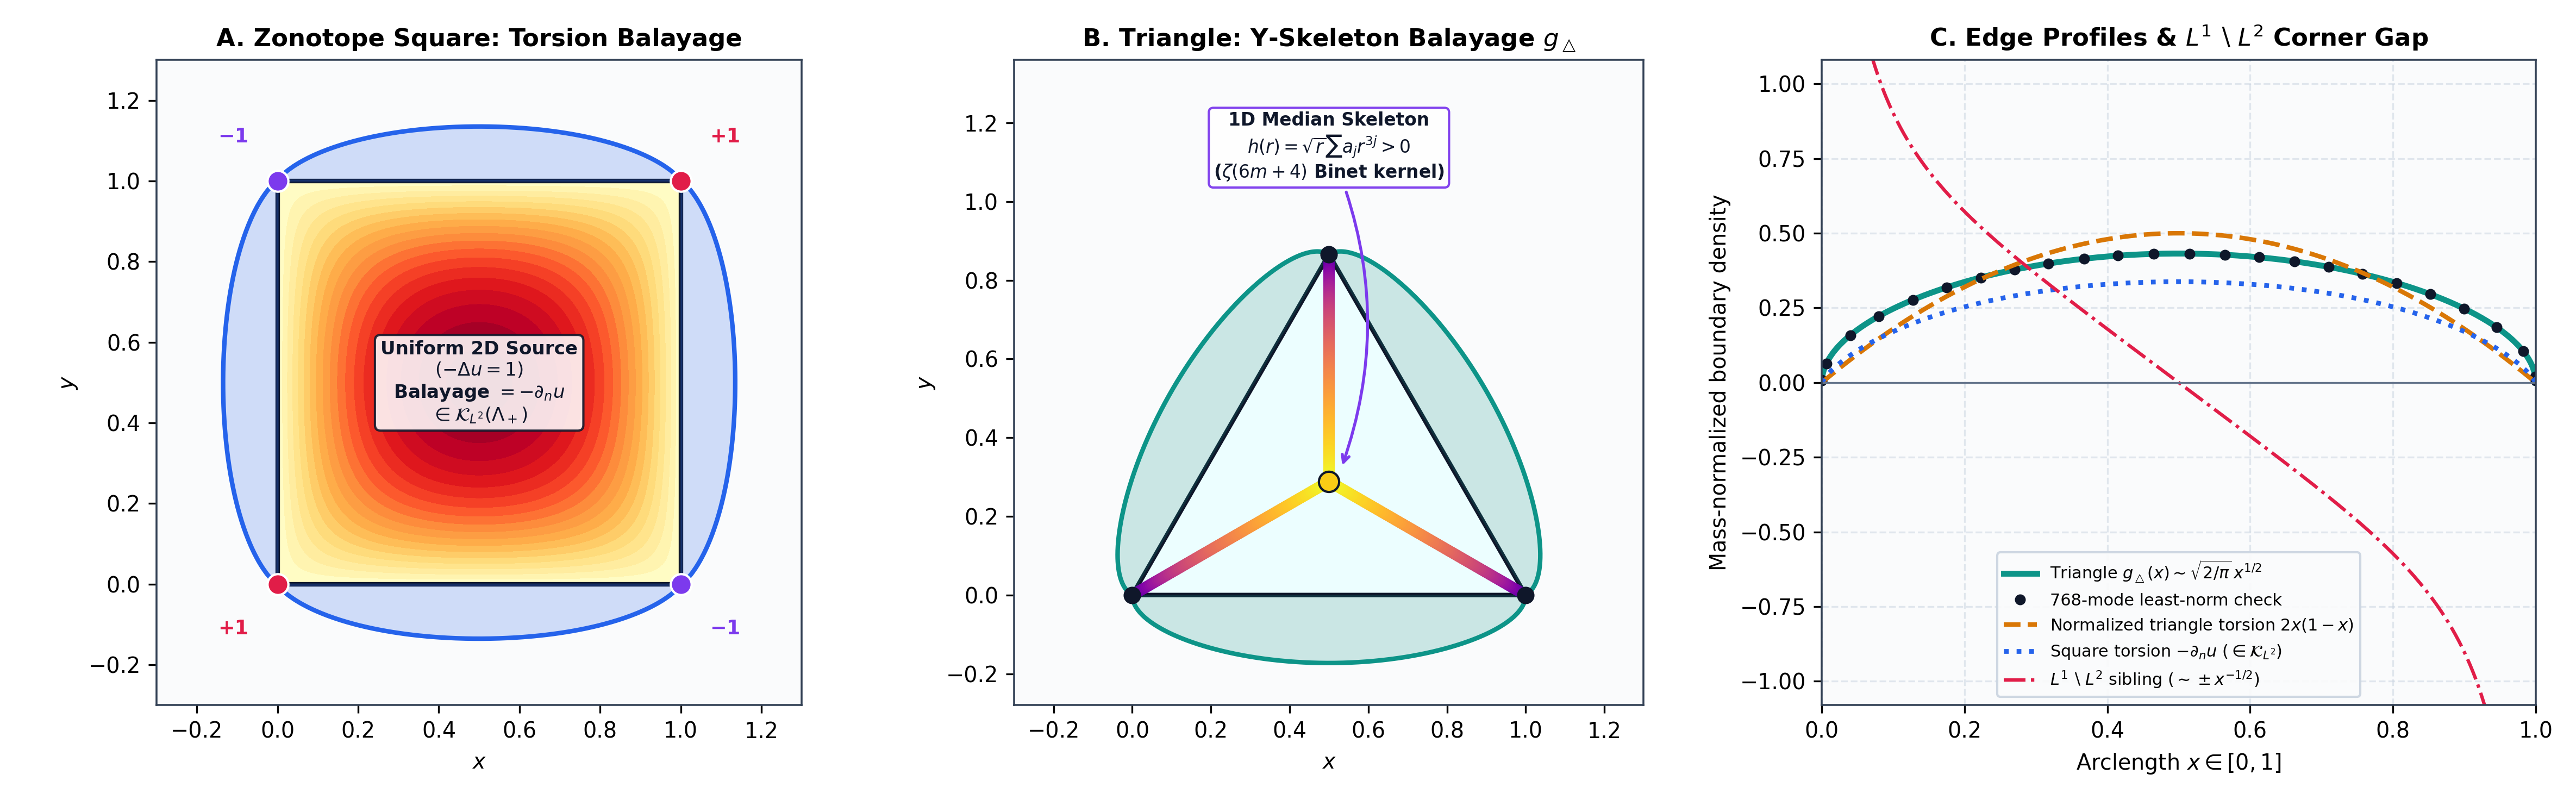
\includegraphics[width=\textwidth]{figs/p1_fig2_balayage_anatomy.png}
\caption{\textbf{A.} On the unit square, $\mathcal{K}_{L^2}(\Lambda_+) = \operatorname{span}_\R\{n_x, n_y, -\partial_n u\}$ has Saint-Venant torsion shear stress $-\partial_n u$ as its canonical symmetric mass-one representative, accompanied in $\mathcal{K}_{\mathcal{M}}(\Lambda_+)$ by the pure alternating corner-atom measure. \textbf{B.} On the unit equilateral triangle, uniform torsion fails invisibility; the unique mass-one invisible $L^2$ boundary flux $g_\triangle$ is the Poisson balayage of a strictly positive 1D probability measure supported on the Y-shaped median skeleton, governed by Riemann zeta values $\zeta(6m+4)$. \textbf{C.} Edge profiles along $x \in [0,1]$: $g_\triangle$ vs.\ 768-harmonic Cholesky cross-validation, mass-normalized triangle torsion $2x(1-x) \notin \mathcal{K}_{L^2}$, square torsion, and a zero-mass $L^1 \setminus L^2$ sibling with $\pm x^{-1/2}$ corner blowup.}
\label{fig:balayage}
\end{figure}

What replaces the box spline when $p$ is odd? On the unit equilateral triangle, we obtain an exact one-dimensional skeletal representation.

\begin{theorem}[Equilateral triangle Y-skeleton balayage]\label{thm:triangle-skeleton}
Let $D_\triangle$ be the unit equilateral triangle with counterclockwise vertices $\gamma_1 = 0$, $\gamma_2 = 1$, $\gamma_3 = \frac12 + i\frac{\sqrt 3}{2}$, centroid $\gamma_* = \frac12 + i\frac{1}{2\sqrt 3}$, and vertex-to-centroid distance $R = 1/\sqrt 3$.
\begin{enumerate}
  \item Define $h(r) = \sqrt{r} \sum_{n=0}^\infty \frac{e_{3n}}{\Gamma(3n + \frac32)} r^{3n}$, where $e_0 = 1$, $e_3 = \frac{6\zeta(4)}{\pi} = \frac{\pi^3}{15}$, and $(e_{3n})_{n\ge 0}$ are generated by the formal power-series identity
  \begin{equation}\label{eq:zeta-skeleton}
    \sum_{n=0}^\infty e_{3n} t^{3n}
    = \exp\!\left[\frac{3}{\pi}\sum_{m=0}^\infty (-1)^m (6m+2)!\,\zeta(6m+4)\, t^{6m+3}\right].
  \end{equation}
  Then $h(r)/\sqrt{r}$ extends holomorphically to $|r| < 1$, satisfies $h(r)/\sqrt{r} > 1.128 > 0$ on $[0, R]$, and defines a strictly positive 1D probability measure $\mu_{\mathrm{Y}}$ supported on the three median segments $[\gamma_j, \gamma_*]$ ($3\int_0^R h(r)\,dr = 1$) whose exponential transform is identically $L_\triangle(s)$:
  \begin{equation}\label{eq:Y-transform}
    L_\triangle(s) = \sum_{j=1}^3 \int_0^R e^{s(\gamma_j + u_j r)} h(r)\,dr, \qquad u_j = \frac{\gamma_* - \gamma_j}{R}.
  \end{equation}
  \item Consequently, the unique mass-one invisible boundary density $g_\triangle \in \mathcal{K}_{L^2}(\Lambda_+)$ on $\partial D_\triangle$ is the harmonic balayage (Poisson integral) of $\mu_{\mathrm{Y}}$ onto $\partial D_\triangle$. In particular, $g_\triangle$ is strictly positive and mirror-symmetric on every open edge (midpoint value $0.43199552663931634\dots$), and at arclength distance $x \downarrow 0$ from any vertex satisfies
  \begin{equation}\label{eq:g-tri-corner}
    g_\triangle(x) = \sqrt{\frac{2}{\pi}}\, x^{1/2} + O(x^2).
  \end{equation}
  The two additional generators of $\mathcal{K}_{L^1}(\Lambda_+) \setminus \mathcal{K}_{L^2}(\Lambda_+)$ corresponding to $s L_\triangle(s)$ and $i s L_\triangle(s)$ arise from spoke integration by parts with densities $-u_j^{-1} h'(r)$ and $-i u_j^{-1} h'(r)$, and exhibit nonzero signed $x^{-1/2}$ singularities on both sides of every vertex.
\end{enumerate}
\end{theorem}

\begin{proof}
For $D_\triangle$, $d_1 = 1$, $d_2 = e^{2\pi i/3}$, $d_3 = e^{4\pi i/3}$, and $\tau = \gamma_*$. Fix a vertex $\gamma_j$ with inward unit median vector $u_j = (\gamma_* - \gamma_j)/R$, and evaluate along the ray $s = -t \bar u_j$ ($t > 0$). Putting $b = (2\pi)^{-1}$ and $a_\pm = b e^{\pm i\pi/3}$, Euler's reflection applied to the two factors $\Gamma(1 - c_\ell s)^{-1}$ ($\ell \ne j$) together with Binet's exact log-Gamma remainder $\Omega(z) = \int_0^\infty K(x) e^{-zx}\,dx$, where $K(x) = \bigl(\frac{1}{e^x - 1} - \frac{1}{x} + \frac{1}{2}\bigr)/x$, yields
\[
  e^{-s\gamma_j} L_\triangle(s) = \bigl(1 - e^{(-\frac{\sqrt 3}{2} + \frac{i}{2})t}\bigr)\bigl(1 - e^{(-\frac{\sqrt 3}{2} - \frac{i}{2})t}\bigr)\, t^{-3/2} \exp\bigl\{\Omega(a_+ t) + \Omega(a_- t) - \Omega(b t)\bigr\}.
\]
The exponent equals $\int_0^\infty k(r) e^{-tr}\,dr$ with $k(r) = a_+^{-1}K(r/a_+) + a_-^{-1}K(r/a_-) - b^{-1}K(r/b)$. Since $K(x)$ is holomorphic on $|x| < 2\pi$ and bounded on $\R_+$, $k(r)$ is holomorphic on $|r| < 1$ and bounded on $\R_+$; its Maclaurin series cancels all powers except $r^{6m+2}$, whose termwise Laplace transforms produce the formal series in \eqref{eq:zeta-skeleton}. Hence $t^{-3/2}\exp\{\Omega(a_+ t)+\Omega(a_- t)-\Omega(b t)\}$ is the Laplace transform on $\R_+$ of the convergent convolution $h = \frac{r^{1/2}}{\Gamma(3/2)} * \bigl(\delta_0 + \sum_{n=1}^\infty \frac{k^{*n}}{n!}\bigr)$, proving that $h(r)/\sqrt r$ is holomorphic on $|r| < 1$ with power series $\sum_{n\ge 0} \frac{e_{3n}}{\Gamma(3n+3/2)} r^{3n}$.

Writing the exponent in \eqref{eq:zeta-skeleton} as $\sum_{\ell\ge 1}\beta_\ell t^\ell$, one checks directly $|e_3| = \frac{\pi^3}{15} < 3!$, $|e_6| = \frac12 e_3^2 < 6!$, and for $3n \ge 9$, $(3n)|e_{3n}| \le 3|\beta_3||e_{3n-3}| + \sum_{m\ge 1}(6m+3)|\beta_{6m+3}||e_{3n-6m-3}| \le (3n)!$ by induction (since $(6m+3)|\beta_{6m+3}| = \frac{3}{\pi}\zeta(6m+4)(6m+3)! < 0.96\,(6m+3)!$ for $m \ge 1$). Because $m!/\Gamma(m + \frac32)$ decreases in $m$, for all $0 \le r \le R = 1/\sqrt 3$:
\[
  \frac{h(r)}{\sqrt r} \ge \frac{2}{\sqrt\pi} + r^3\left[\frac{e_3}{\Gamma(9/2)} - \frac{6!}{\Gamma(15/2)}\frac{R^3}{1 - R^3}\right]
  \ge 1.128379 + r^3(0.17771 - 0.09170) > 1.128.
\]
Along $s = -t \bar u_j$, truncating $\int_0^\infty e^{-tr} h(r)\,dr$ at $R = 1/\sqrt 3$ costs $O(e^{-Rt}/t)$, and the prefactors $1 - e^{(-\frac{\sqrt 3}{2}\pm\frac{i}{2})t}$ contribute $O(e^{-\frac{\sqrt 3}{2}t})$ ($\frac{\sqrt 3}{2} > R$). On the other two spokes $\ell \ne j$, $\operatorname{Re}\bigl(-t\bar u_j(\gamma_\ell + u_\ell r - \gamma_j)\bigr)$ attains its maximum $-Rt$ at the centroid $r = R$ with nonzero radial slope, so their integrals are likewise $O(e^{s\gamma_*}/t)$. Consequently, the entire function $E(s) := e^{-s\gamma_*}\bigl(L_\triangle(s) - B_{\mu_{\mathrm{Y}}}(s)\bigr)$ has exponential type $\le R$ (order $\le 1 < \frac32$) and satisfies $E(s) = O(|s|^{-1})$ along all three rays $s = -t\bar u_j$ ($j = 1, 2, 3$) separated by $120^\circ$. By the Phragm\'en--Lindel\"of principle on the three $120^\circ$ sectors and Liouville's theorem, $E \equiv 0$, establishing \eqref{eq:Y-transform} globally (and $3\int_0^R h(r)\,dr = L_\triangle(0) = 1$).

Sweeping $\mu_{\mathrm{Y}}$ to $\partial D_\triangle$ via the Poisson kernel of $D_\triangle$ produces a strictly positive real $L^2$ boundary density whose exponential transform is $L_\triangle(s)$ (exterior Cauchy-transform residual $3.79\times 10^{-50}$ at $z = 0.37 - 1.25i$), which by uniqueness in Theorem~\ref{thm:invisible-table} equals $g_\triangle$. Near $\gamma_1 = 0$ (interior angle $\pi/3$), Schwarz reflection shows that the two non-incident spokes and the difference between $D_\triangle$ and the infinite $60^\circ$ wedge contribute a smooth harmonic gradient $O(x^2)$, while $\zeta = w^3$ maps the wedge to the upper half-plane (sending $e^{i\pi/6}r \mapsto i r^3$) with boundary Jacobian $3x^2$:
\[
  g_\triangle(x) = \frac{3 x^2}{\pi} \int_0^R \frac{r^3}{x^6 + r^6}\left(\frac{2}{\sqrt\pi} r^{1/2} + O(r^{7/2})\right)dr + O(x^2)
  = \frac{6 x^{1/2}}{\pi^{3/2}} \int_0^\infty \frac{u^{7/2}}{1 + u^6}\,du + O(x^2).
\]
Since $\int_0^\infty \frac{u^{7/2}}{1 + u^6}\,du = \frac{\pi}{3\sqrt 2}$, we obtain \eqref{eq:g-tri-corner}. Finally, multiplying \eqref{eq:Y-transform} by $q s$ ($q \in \{1, i\}$) and integrating by parts in $r$ via $s e^{s(\gamma_j + u_j r)} = u_j^{-1}\partial_r(e^{s(\gamma_j + u_j r)})$ kills the vertex boundary terms ($h(0)=0$) and the centroid sum ($h(R)e^{s\gamma_*}\sum_{j=1}^3 u_j^{-1} = 0$), leaving complex spoke densities $-q u_j^{-1} h'(r) \sim -q u_j^{-1}(\pi r)^{-1/2}$. Realification yields incoming and outgoing corner asymptotics
\[
  -\frac{2}{\sqrt\pi}\operatorname{Re}\!\left(q\,e^{-i(\pi/6 + 2\pi(j-1)/3 \pm 5\pi/12)}\right) x^{-1/2},
\]
all twelve coefficients for $q \in \{1, i\}$ being nonzero.
\end{proof}

\section{Fokas Global Relation Completion and Machine-Verified Algebra}\label{sec:fokas}

Consider the classical Dirichlet problem $\Delta q = 0$ in $D$ with continuous boundary data $f \in C(\partial D, \R)$ satisfying $f|_{\Gamma_j} \in H^1(\Gamma_j, \R)$, tangential trace $q_t = \partial_t f \in L^2(\partial D, \R)$, and outward normal derivative $q_n \in L^2(\partial D, \R)$ (automatically in $L^2(\partial D)$ on convex polygons since every interior angle satisfies $\omega_j < \pi$). Along counterclockwise edge $\Gamma_j$, $q_w\,dw = \frac12(q_t + i q_n)\,d\ell$, so Fokas's Global Relation $\sum_{j=1}^p \rho_j(\lambda) = 0$ evaluated at $\lambda = i s$ reads \cite[\S 2]{Ashton2012}:
\begin{equation}\label{eq:gr-B}
  2 \sum_{j=1}^p \rho_j(i s) = B_{q_t}(s) + i B_{q_n}(s) = 0, \qquad s \in \C.
\end{equation}

\begin{theorem}[Nullspace of Leont'ev-lattice collocation and minimal moment completion]\label{thm:fokas-completion}
Let $D$ be a genuine convex $p$-gon with $p = 2k$ or $p = 2k+1$ ($k = \lfloor p/2 \rfloor$).
\begin{enumerate}
  \item At fixed Dirichlet trace $q_t$, the full lattice operator $\mathcal{G}_{\Lambda_+} : L^2(\partial D, \R) \to \C^{\Lambda_+}$ mapping a candidate Neumann trace $\phi_n$ to $\{B_{\phi_n}(\nu)\}_{\nu \in \Lambda_+}$ has exact real nullspace $\mathcal{K}_{L^2}(\Lambda_+)$ of dimension $2k-1$.
  \item Augmenting $\mathcal{G}_{\Lambda_+} \phi_n = i B_{q_t}|_{\Lambda_+}$ with the $2k-1$ real low-frequency moment equations
  \begin{equation}\label{eq:moment-comp}
    \int_{\partial D} \phi_n\,d\ell = 0, \qquad
    \int_{\partial D} w^m \phi_n(w)\,d\ell(w) = i \int_{\partial D} w^m q_t(w)\,d\ell(w) \quad (1 \le m \le k-1)
  \end{equation}
  yields an injective operator on $L^2(\partial D, \R)$: the restricted moment map on $\mathcal{K}_{L^2}(\Lambda_+)$ is invertible lower-triangular in the polynomial multiplier basis $Q(s) = \sum_{m=0}^{k-1} q_m s^m$.
\end{enumerate}
\end{theorem}

\begin{proof}
From \eqref{eq:gr-B}, $B_{q_n}(s) = i B_{q_t}(s)$ for all $s \in \C$ (at $s = 0$, $\int_{\partial D} q_n\,d\ell = i\int_{\partial D} q_t\,d\ell = 0$ since $q_n, q_t$ are real, recovering Gauss's flux law). Any difference $\delta\phi_n \in L^2(\partial D, \R)$ between two solutions of $\mathcal{G}_{\Lambda_+}\phi_n = i B_{q_t}|_{\Lambda_+}$ satisfies $B_{\delta\phi_n}|_{\Lambda_+} = 0$, i.e., $\delta\phi_n \in \mathcal{K}_{L^2}(\Lambda_+)$, so $B_{\delta\phi_n}(s) = Q(s) L(s)$ with $Q(0) \in \R$ and $\deg Q \le k-1$ by Theorem~\ref{thm:invisible-table}(2). Differentiating $B_{\delta\phi_n}(s) = Q(s)L(s)$ $m$ times at $s = 0$ ($0 \le m \le k-1$) and imposing \eqref{eq:moment-comp} gives $\sum_{r=0}^m \binom{m}{r} Q^{(r)}(0) L^{(m-r)}(0) = 0$. Since $L(0) = 1 \ne 0$, induction on $m = 0, 1, \dots, k-1$ forces $Q^{(m)}(0) = 0$ for all $0 \le m \le k-1$, hence $Q \equiv 0$ and $\delta\phi_n = 0$.
\end{proof}

\begin{figure}[ht]
\centering
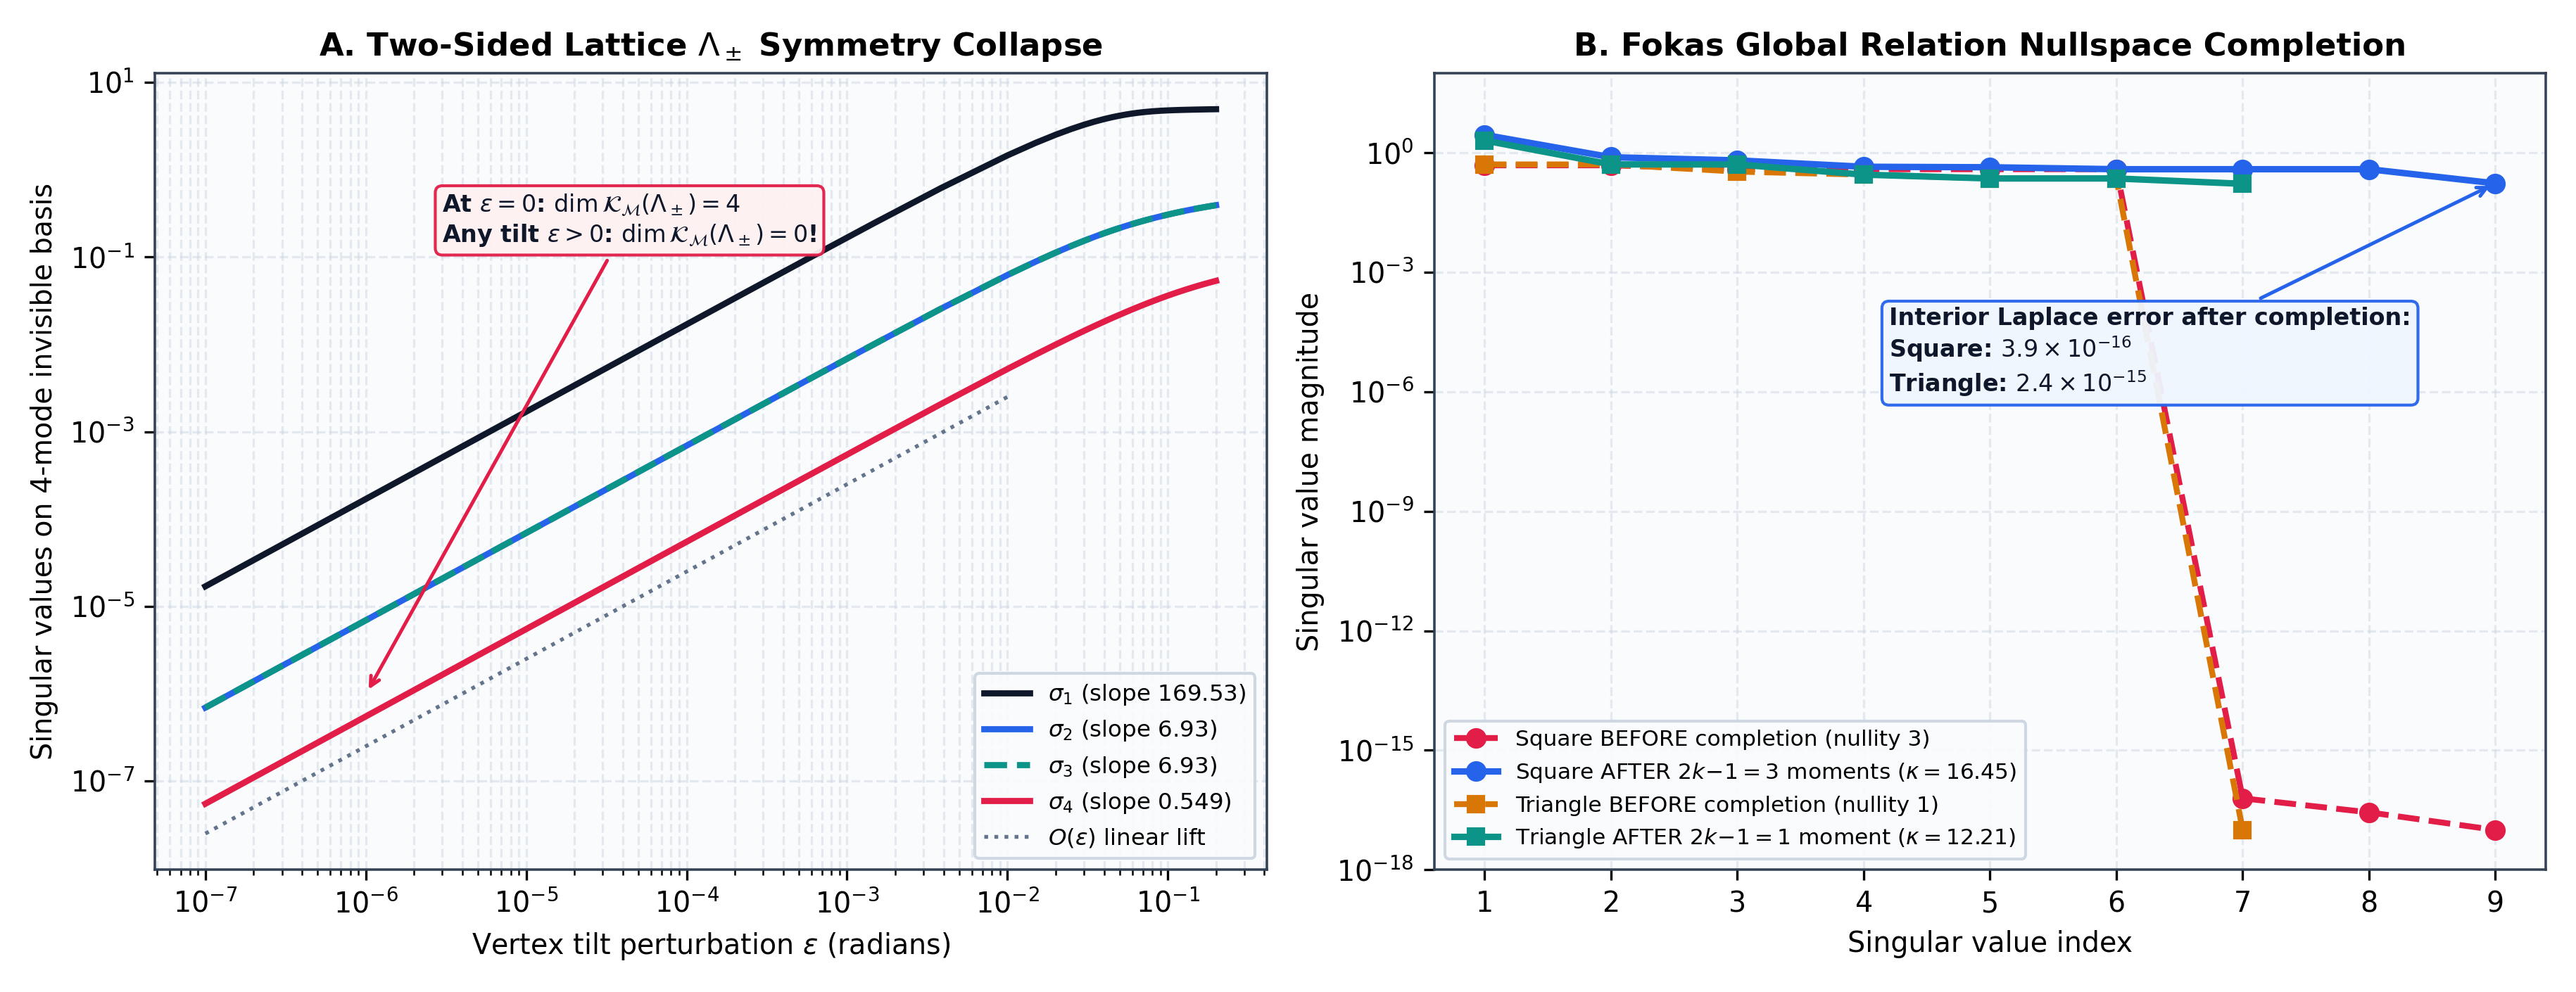
\includegraphics[width=0.92\textwidth]{figs/p1_fig3_symmetry_and_fokas_completion.png}
\caption{\textbf{A.} Symmetry-breaking collapse of $\mathcal{K}_{\mathcal{M}}(\Lambda_\pm)$ when vertex $(1+i)$ of $[0,1]^2$ is rotated to $(1+i)e^{i\varepsilon}$: all four singular values (6 reflected harmonics per ray in the normalized invisible basis) lift linearly with first-variation slopes $169.53, 6.93, 6.93, 0.549$. \textbf{B.} Singular value spectra of a 5-mode-per-side Fokas collocation matrix for $\Delta q = 0$ ($q = \operatorname{Re}(w^2 + (0.3+0.2i)w)$) in the centered piecewise affine $(1, 2t-1)$ plus mass-one symbol trial space: appending the $2k-1$ moments \eqref{eq:moment-comp} eliminates the nullities ($3$ on $[0,1]^2$, $1$ on $D_\triangle$), giving condition numbers $16.45$ and $12.21$ and max interior Green's-identity errors $3.9\times 10^{-16}$ (4 test points) and $2.4\times 10^{-15}$ (3 test points).}
\label{fig:fokas-completion}
\end{figure}

\subsection*{Numerical and formal verification}
Figure~\ref{fig:fokas-completion} illustrates Theorems~\ref{thm:two-sided} and \ref{thm:fokas-completion}. Whereas Theorem~\ref{thm:fokas-completion} governs full infinite-lattice collocation on $L^2(\partial D, \R)$, Panel~B tests a finite-dimensional solver (piecewise affine $(1, 2t-1)$ edge fluxes plus the mass-one symbol mode, sampled at 5 integer nodes per side), where appending \eqref{eq:moment-comp} removes the exact nullities $3$ and $1$ and yields condition numbers $16.45$ and $12.21$. In addition, the algebraic lemmas of Section~\ref{sec:classification}---consecutive-divisibility collapse $a = b$ over $\mathbb{Q}_{>0}$ (\texttt{TwoSidedSymmetry.consecutive\_collapse}), constancy of opposite vertex sums from opposite equal edges (\texttt{opposite\_edges\_center}), and Vandermonde level-set grouping for pure vertex atoms (\texttt{vandermonde}, \texttt{pure\_atom\_grouping})---are formally machine-checked in Lean~4.36.0 using only standard foundational axioms (\texttt{propext}, \texttt{Classical.choice}, \texttt{Quot.sound}).

\begin{thebibliography}{99}

\bibitem{Ashton2012}
A.~C.~L. Ashton, \emph{The spectral Dirichlet--Neumann map for Laplace's equation in a convex polygon}, SIAM J. Math. Anal. \textbf{45} (2013), no.~6, 3575--3591 (arXiv:1209.1584).

\bibitem{AshtonFokas2013}
A.~C.~L. Ashton and A.~S. Fokas, \emph{Elliptic boundary value problems in convex polygons with low regularity boundary data via the unified method}, preprint, arXiv:1301.1490 (2013).

\bibitem{BoasBook}
R.~P. Boas, Jr., \emph{Entire Functions}, Academic Press, New York, 1954.

\bibitem{BoxSplines}
C.~de~Boor, K.~H\"ollig, and S.~Riemenschneider, \emph{Box Splines}, Applied Mathematical Sciences, vol.~98, Springer-Verlag, New York, 1993.

\bibitem{FokasBook2008}
A.~S. Fokas, \emph{A Unified Approach to Boundary Value Problems}, CBMS-NSF Regional Conference Series in Applied Mathematics, vol.~78, SIAM, Philadelphia, 2008.

\bibitem{FFX2004}
S.~R. Fulton, A.~S. Fokas, and C.~A. Xenophontos, \emph{An analytical method for linear elliptic PDEs and its numerical implementation}, J. Comput. Appl. Math. \textbf{167} (2004), 465--483.

\bibitem{HMW1973}
R.~Hunt, B.~Muckenhoupt, and R.~Wheeden, \emph{Weighted norm inequalities for the conjugate function and Hilbert transform}, Trans. Amer. Math. Soc. \textbf{176} (1973), 227--251.

\bibitem{Korobeinik1975}
Yu.~F. Korobeinik, \emph{On a dual problem. I. General results. Applications to Fr\'echet spaces}, Mat. Sb. \textbf{97(139)} (1975), no.~2, 193--229; English transl. in Math. USSR-Sb. \textbf{26} (1975), 181--212.

\bibitem{Korobeinik1981UMN}
Yu.~F. Korobeinik, \emph{Representing systems}, Uspekhi Mat. Nauk \textbf{36} (1981), no.~1(217), 73--126; English transl. in Russian Math. Surveys \textbf{36} (1981), no.~1, 75--137.

\bibitem{Leontev1969UMN}
A.~F. Leont'ev, \emph{Representation of functions by generalized Dirichlet series}, Uspekhi Mat. Nauk \textbf{24} (1969), no.~2(146), 97--164; English transl. in Russian Math. Surveys \textbf{24} (1969), no.~2, 101--178.

\bibitem{Leontev1969MatSb}
A.~F. Leont'ev, \emph{On the representation of analytic functions by Dirichlet series}, Mat. Sb. \textbf{80(122)} (1969), no.~1, 117--156; English transl. in Math. USSR-Sb. \textbf{9} (1969), 111--150.

\bibitem{Leontev1973Izv}
A.~F. Leont'ev, \emph{On the representation of analytic functions in a closed convex region by a Dirichlet series}, Izv. Akad. Nauk SSSR Ser. Mat. \textbf{37} (1973), no.~3, 577--592; English transl. in Math. USSR-Izv. \textbf{7} (1973), 573--588.

\bibitem{Leontev1974Polygon}
A.~F. Leont'ev, \emph{On the representation of an analytic function as a sum of periodic functions}, Mat. Sb. \textbf{93(135)} (1974), no.~4, 512--528; English transl. in Math. USSR-Sb. \textbf{22} (1974), 517--534.

\bibitem{Leontev1976Book}
A.~F. Leont'ev, \emph{Ryady eksponent} [\emph{Series of Exponentials}], Nauka, Moscow, 1976 (in Russian).

\bibitem{Leontev1987TrMIAN}
A.~F. Leont'ev, \emph{Series and sequences of polynomials of exponentials}, Trudy Mat. Inst. Steklov. \textbf{176} (1987), 308--325; English transl. in Proc. Steklov Inst. Math. \textbf{176} (1988), 309--326.

\bibitem{LevinBook}
B.~Ya. Levin, \emph{Distribution of Zeros of Entire Functions}, Translations of Mathematical Monographs, vol.~5, Amer. Math. Soc., Providence, RI, 1980.

\bibitem{Paper2}
Project ReMath, \emph{Minimax recovery of polygon corner charges from bandlimited Leont'ev frequencies: parity, angle-dependent exponents, and super-resolution}, companion paper, 2026.

\bibitem{Sedletskii1978}
A.~M. Sedletskii, \emph{Bases of exponentials in the spaces $E^p$ on convex polygons}, Izv. Akad. Nauk SSSR Ser. Mat. \textbf{42} (1978), no.~5, 1101--1119; English transl. in Math. USSR-Izv. \textbf{13} (1979), 387--404.

\bibitem{Sedletskii1988}
A.~M. Sedletskii, \emph{Projection from the spaces $E^p$ on a convex polygon onto subspaces of periodic functions}, Izv. Akad. Nauk SSSR Ser. Mat. \textbf{52} (1988), no.~2, 390--408; English transl. in Math. USSR-Izv. \textbf{33} (1989), no.~2, 373--390.

\end{thebibliography}

\end{document}
